\documentclass[]{book}
\usepackage{lmodern}
\usepackage{amssymb,amsmath}
\usepackage{ifxetex,ifluatex}
\usepackage{fixltx2e} % provides \textsubscript
\ifnum 0\ifxetex 1\fi\ifluatex 1\fi=0 % if pdftex
  \usepackage[T1]{fontenc}
  \usepackage[utf8]{inputenc}
\else % if luatex or xelatex
  \ifxetex
    \usepackage{mathspec}
  \else
    \usepackage{fontspec}
  \fi
  \defaultfontfeatures{Ligatures=TeX,Scale=MatchLowercase}
\fi
% use upquote if available, for straight quotes in verbatim environments
\IfFileExists{upquote.sty}{\usepackage{upquote}}{}
% use microtype if available
\IfFileExists{microtype.sty}{%
\usepackage[]{microtype}
\UseMicrotypeSet[protrusion]{basicmath} % disable protrusion for tt fonts
}{}
\PassOptionsToPackage{hyphens}{url} % url is loaded by hyperref
\usepackage[unicode=true]{hyperref}
\hypersetup{
            pdftitle={Bio 373L Survival Guide},
            pdfauthor={Christopher R. Peterson},
            pdfborder={0 0 0},
            breaklinks=true}
\urlstyle{same}  % don't use monospace font for urls
\usepackage{natbib}
\bibliographystyle{apalike}
\usepackage{color}
\usepackage{fancyvrb}
\newcommand{\VerbBar}{|}
\newcommand{\VERB}{\Verb[commandchars=\\\{\}]}
\DefineVerbatimEnvironment{Highlighting}{Verbatim}{commandchars=\\\{\}}
% Add ',fontsize=\small' for more characters per line
\usepackage{framed}
\definecolor{shadecolor}{RGB}{248,248,248}
\newenvironment{Shaded}{\begin{snugshade}}{\end{snugshade}}
\newcommand{\KeywordTok}[1]{\textcolor[rgb]{0.13,0.29,0.53}{\textbf{#1}}}
\newcommand{\DataTypeTok}[1]{\textcolor[rgb]{0.13,0.29,0.53}{#1}}
\newcommand{\DecValTok}[1]{\textcolor[rgb]{0.00,0.00,0.81}{#1}}
\newcommand{\BaseNTok}[1]{\textcolor[rgb]{0.00,0.00,0.81}{#1}}
\newcommand{\FloatTok}[1]{\textcolor[rgb]{0.00,0.00,0.81}{#1}}
\newcommand{\ConstantTok}[1]{\textcolor[rgb]{0.00,0.00,0.00}{#1}}
\newcommand{\CharTok}[1]{\textcolor[rgb]{0.31,0.60,0.02}{#1}}
\newcommand{\SpecialCharTok}[1]{\textcolor[rgb]{0.00,0.00,0.00}{#1}}
\newcommand{\StringTok}[1]{\textcolor[rgb]{0.31,0.60,0.02}{#1}}
\newcommand{\VerbatimStringTok}[1]{\textcolor[rgb]{0.31,0.60,0.02}{#1}}
\newcommand{\SpecialStringTok}[1]{\textcolor[rgb]{0.31,0.60,0.02}{#1}}
\newcommand{\ImportTok}[1]{#1}
\newcommand{\CommentTok}[1]{\textcolor[rgb]{0.56,0.35,0.01}{\textit{#1}}}
\newcommand{\DocumentationTok}[1]{\textcolor[rgb]{0.56,0.35,0.01}{\textbf{\textit{#1}}}}
\newcommand{\AnnotationTok}[1]{\textcolor[rgb]{0.56,0.35,0.01}{\textbf{\textit{#1}}}}
\newcommand{\CommentVarTok}[1]{\textcolor[rgb]{0.56,0.35,0.01}{\textbf{\textit{#1}}}}
\newcommand{\OtherTok}[1]{\textcolor[rgb]{0.56,0.35,0.01}{#1}}
\newcommand{\FunctionTok}[1]{\textcolor[rgb]{0.00,0.00,0.00}{#1}}
\newcommand{\VariableTok}[1]{\textcolor[rgb]{0.00,0.00,0.00}{#1}}
\newcommand{\ControlFlowTok}[1]{\textcolor[rgb]{0.13,0.29,0.53}{\textbf{#1}}}
\newcommand{\OperatorTok}[1]{\textcolor[rgb]{0.81,0.36,0.00}{\textbf{#1}}}
\newcommand{\BuiltInTok}[1]{#1}
\newcommand{\ExtensionTok}[1]{#1}
\newcommand{\PreprocessorTok}[1]{\textcolor[rgb]{0.56,0.35,0.01}{\textit{#1}}}
\newcommand{\AttributeTok}[1]{\textcolor[rgb]{0.77,0.63,0.00}{#1}}
\newcommand{\RegionMarkerTok}[1]{#1}
\newcommand{\InformationTok}[1]{\textcolor[rgb]{0.56,0.35,0.01}{\textbf{\textit{#1}}}}
\newcommand{\WarningTok}[1]{\textcolor[rgb]{0.56,0.35,0.01}{\textbf{\textit{#1}}}}
\newcommand{\AlertTok}[1]{\textcolor[rgb]{0.94,0.16,0.16}{#1}}
\newcommand{\ErrorTok}[1]{\textcolor[rgb]{0.64,0.00,0.00}{\textbf{#1}}}
\newcommand{\NormalTok}[1]{#1}
\usepackage{longtable,booktabs}
% Fix footnotes in tables (requires footnote package)
\IfFileExists{footnote.sty}{\usepackage{footnote}\makesavenoteenv{long table}}{}
\usepackage{graphicx,grffile}
\makeatletter
\def\maxwidth{\ifdim\Gin@nat@width>\linewidth\linewidth\else\Gin@nat@width\fi}
\def\maxheight{\ifdim\Gin@nat@height>\textheight\textheight\else\Gin@nat@height\fi}
\makeatother
% Scale images if necessary, so that they will not overflow the page
% margins by default, and it is still possible to overwrite the defaults
% using explicit options in \includegraphics[width, height, ...]{}
\setkeys{Gin}{width=\maxwidth,height=\maxheight,keepaspectratio}
\IfFileExists{parskip.sty}{%
\usepackage{parskip}
}{% else
\setlength{\parindent}{0pt}
\setlength{\parskip}{6pt plus 2pt minus 1pt}
}
\setlength{\emergencystretch}{3em}  % prevent overfull lines
\providecommand{\tightlist}{%
  \setlength{\itemsep}{0pt}\setlength{\parskip}{0pt}}
\setcounter{secnumdepth}{5}
% Redefines (sub)paragraphs to behave more like sections
\ifx\paragraph\undefined\else
\let\oldparagraph\paragraph
\renewcommand{\paragraph}[1]{\oldparagraph{#1}\mbox{}}
\fi
\ifx\subparagraph\undefined\else
\let\oldsubparagraph\subparagraph
\renewcommand{\subparagraph}[1]{\oldsubparagraph{#1}\mbox{}}
\fi

% set default figure placement to htbp
\makeatletter
\def\fps@figure{htbp}
\makeatother

\usepackage{booktabs}

\title{Bio 373L Survival Guide}
\author{Christopher R. Peterson}
\date{2020-01-29}

\begin{document}
\maketitle

{
\setcounter{tocdepth}{1}
\tableofcontents
}
\chapter*{Preface}\label{preface}
\addcontentsline{toc}{chapter}{Preface}

This book contains advice for students in the University of Texas at
Austin's Field Ecology course. It will be updated throughout the
semester. The first three chapters contain general guidelines for
writing lab reports.

\chapter{Writing Lab Reports: Structure}\label{structure}

\section{Structure Overview}\label{structure-overview}

The main goal of scientific writing is to effectively communicate
complicated concepts. Scientific manuscripts tend to follow a
traditional structure that is intended to help an experienced reader
navigate these concepts. Each section should answer a question:

\begin{itemize}
\tightlist
\item
  \textbf{Abstract}: Why should I read this?
\item
  \textbf{Introduction}: Why did you do this?\\
\item
  \textbf{Methods}: What did you do and where/with what did you do it?
\item
  \textbf{Results}: What did you find?\\
\item
  \textbf{Discussion}: What does it mean and why does it matter?
\item
  \textbf{Literature Cited}: Doesn't really answer a question, but this
  is where you list the citations you used.
\end{itemize}

Greater detail is provided in the following sections.

\section{Abstract}\label{abstract}

The abstract is a one paragraph summary that functions as an
advertisement/elevator pitch for the rest of the paper. A reader should
get a general idea about what you did and be interested in reading the
rest of the paper. If it's more than 350 words, you need to shorten it.

While this section should cover the intro, methods, results, and
discussion, you shouldn't re-use any language from those sections here.
Instead, write a sentence or two from each that hits the important
points without going into all of the details. Don't cite any figures,
tables, or other literature in here.

Generally, this section is written last.

\section{Introduction}\label{introduction}

The introduction section sets the stage for the work you are about to
describe and should tell your reader \emph{why} your research is
interesting. You should begin by describing the broader ecological
context that your research fits into, and review the relevant
literature. It is a good idea to start generally and narrow the focus to
the specific project you did.

For example, let's say you're writing a paper about the temperature
tolerance of the three-eyed sandslider (\emph{Trioptis cerastes}), a
fictional snake species we're going to pretend is native to southwestern
deserts. A reasonable introduction could discuss the following:

\begin{itemize}
\tightlist
\item
  Climate change in general.
\item
  Severity and effects of climate change in deserts.
\item
  Effects of higher temperature on ectotherm behavior.
\item
  How you're investigating temperature tolerance with three-eyed
  sandslider.
\end{itemize}

Alternatively, you could introduce the same paper in a completely
different context:

\begin{itemize}
\tightlist
\item
  The evolution of animal activity budgets.
\item
  Effects of temperature on foraging and reproductive behavior in
  ectotherms.
\item
  How you're investigating temperature tolerance with three-eyed
  sandslider.
\end{itemize}

There are many more potential ways to write this paper. The take home
message is to set your specific project within the bigger picture of a
large-scale concept, phenomenon, or issue.

The introduction should contain at least two paragraphs (with a minimum
of three sentences each). At the end of the section, you should
explicitly state your hypotheses and predictions. For example, going
back to the temperature tolerance experiment, I could write, `Thus, I
hypothesize that \emph{Trioptis cerastes} will have a higher temperature
tolerance in the summer than in the winter due to acclimation to higher
temperatures in the warmer months''.

You should cite at least two peer-reviewed papers in this section.
Please ensure these papers are actually relevant to what you're talking
about and aren't just tacked on to meet this requirement.

\section{Methods}\label{methods}

This section includes detailed information on your experimental setup,
data collection procedures, and the statistical analyses you used. If
your project focused on specific species or sites (e.g., BFL), you
should start by describing these.

It is often useful to organize the methods section into sub-sections.
For example, for the temperature tolerance example could have the
following sub-sections:

\begin{itemize}
\tightlist
\item
  Study Region
\item
  Study Organism
\item
  Housing Conditions
\item
  Experimental Design
\item
  Statistical Analyses
\end{itemize}

You should always include a description of \emph{all} of the statistical
methods you used in the methods section. This includes the test(s)
performed, the predictor (independent) and response (dependent)
variables, the alpha level, and the program used.

Write each sub-section in chronological order. This and the results
section are often the easiest to write first, so it's best to start with
these two middle sections, and then work on the introduction and
discussion.

\section{Results}\label{results}

This is where you describe your observations and the results of any
analyses. Make sure you do not include new methods (\textbf{including
new statistical analyses}) in this section; these belong in the previous
section. The most important results should be presented as figures or
tables. However, they must also be described in the paragraph.

It is a good idea to organize this section into sub-sections as well,
following the same system you used in the methods (some sub-sections
from the methods may not need to be used in the results, but follow the
organization as closely as possible).

\subsection{Reporting statistics}\label{reporting-statistics}

In general, you should begin by presenting the relevant summary
statistics (such as means for measured data and frequencies for
categorical data). For example, `The mean temperature tolerance was
\(39.2 \pm 0.45 ºC\) for males and \(37.1 \pm 0.25 ºC\) for females.'
Notice that the temperature has units (degrees Celsius) and that I put
the standard deviation after the mean. This is good practice when
reporting means.

When reporting statistical test results, state what they mean in words
first, and then follow the statement with a parenthetical phrase
containing the statistics. For example, `Males tolerated significantly
higher temperatures than females (\(t = 1.96\), \(df = 6\),
\(p = 0.04\))'. Notice that I included the computed t-statistic, the
degrees of freedom and the p-value. All these should be reported when
reporting t-test results. Note also that I indicated the direction of
the difference, as well as its significance.

Here is another example: `The number of escape behaviors performed
increased significantly at high temperatures for all snakes
(\(\chi^2 = 8.43\), \(df = 2\), \(p = 0.001\))'. This is an example of
how you would report chi-square test results. Again, the results are
stated in words that have biological meaning and are followed by the
calculated test statistic, the degrees of freedom and the p-value in
parentheses.

If your statistical analyses did not find a significant difference, you
still need to report this. For example: `Although temperature tolerance
was slightly higher for males than females, this difference was not
statistically significant (\(t = 0.657\), \(df = 6\), \(p = 0.14\)).' Do
not use the word ``insignificant'' in this context.

\emph{Be sure to state your results in a biologically meaningful
manner.} A common mistake is to write out the results in statistical
terminology without any reference to their biological meaning. For
example: `A t-test resulted in a p-value of 0.03 meaning that we can
reject the null hypothesis and accept the alternative.' While this is a
correct statistical interpretation of the calculated p-value, it tells
the reader nothing about the trees or ants or mushrooms that you were
studying. Do not write up your results like this; it's unpleasant to
read and you're just going to have to fix it in revisions.

\subsection{Do not interpret your data
here}\label{do-not-interpret-your-data-here}

Do not interpret your data in the results. That belongs in the
discussion.

Do not consider explanations for your data in the results. That belongs
in the discussion.

Do not consider how your data relates to your hypothesis in the results.
That belongs in the discussion.

This is probably the most common mistake I've encountered in grading
student lab reports.

\section{Discussion}\label{discussion}

The discussion is where you should interpret your data and draw
conclusions by comparing your data to what is known from the published
literature. The organization of this section is a mirror-image of the
introduction in terms of its organization: start narrowly, by discussing
how your results relate to your original hypotheses and questions.
Follow it up with a wider discussion of how these results fit into the
broad concept with which you introduced the paper. This should not be a
restatement of what you wrote in the introduction or in the results, but
should be an exploration of the meaning of all those numbers you just
crunched and what they might signify.

Be careful not to make unfounded statements. There are often many
potential explanations for obtaining a particular result. One may seem
more likely than the others, but this does not exclude the other
explanations from being true if you haven't actually tested them. A good
way to handle this is to mention the multiple alternative
interpretations, express support for the one you think is most likely
and explain why, then suggest a future experiment that could be done to
test whether or not that is correct.

An example:

\begin{quote}
`Temperature tolerance was lower for females than for males. This could
be due to the relative size of the two sexes. Females are the smaller
sex, meaning that they would heat up faster than males due to a greater
surface area:volume ratio (Loblaw and Bluth, 2005). Alternatively, the
males could have a higher tolerance because their overall activity
levels were elevated in the experimental enclosures. This may have
caused them to begin with a higher internal temperature that
acclimatized them to higher temperatures to start; however, this seems
unlikely. Future work could address this by taking internal temperature
readings before and after temperature tolerance trials.'
\end{quote}

As in the introduction, you should cite at least two peer-reviewed
papers in this section in a way that isn't obviously shoehorned in.

\section{Literature Cited}\label{literature-cited}

You must use a minimum of \textbf{four} primary literature sources in
your report, with at least two sources in both the introduction and
discussion (although some sources are suitable to use in both). Use the
sources to provide background, to aid in justification of performing the
project, support for your interpretation of results, etc. In some cases,
you should also cite a reference in the methods section (e.g., for a
non-standard data collection technique or to provide information on a
study site/species). Do not cite papers in results. All thoughts, ideas,
concepts, etc., that you didn't think up on your own must be cited in
the text (failure to do this is considered plagiarism).

If you want to cite general facts or information from a study, it's
generally best to present those facts with a parenthetical citation.
E.g., ``The point-quarter technique is an effective and reliable way to
estimate canopy cover in the field (Smith et al., 2018).'' Sometimes,
you may want to discuss the specific details of a previous paper.
Generally, it's a bad idea to start a sentence with ``In one study,
\ldots{} (Hernandez et al., 2007). Instead, cite them
directly:''Hernandez et al. (2007) discovered similar signs of
succession in eastern hardwood forests\ldots{}``. If you have multiple
sentences all drawn from the same source, just put the citation once at
the end of the last of those sentences.

Please note that while there is a minimum of four primary literature
sources, you are encouraged to add more. Bringing in information from
extra papers can really strengthen your introduction/discussion. There
will be a weekly thread on Canvas to share literature relevant to the
lab report; you are expected to contribute two citations to it each
week.

Please note that your sources need to be relevant to your lab report at
more than just a surface level. For example, if your lab report is on
the distribution of cottonwoods at BFL, a paper about the cottonwood's
genomic structure is probably not going to be relevant.

\section{Common Mistakes for particular
sections}\label{common-mistakes-for-particular-sections}

\subsection{Introduction and
Discussion}\label{introduction-and-discussion}

Null hypotheses are statistical tools used for certain tests (e.g., a
null hypothesis for a chi-squared test would be that the groups are
independent, or that there is no difference in the species proportions
between the two age classes). These don't belong in the introduction or
discussion. For these sections, you should present your biological
hypotheses (e.g., ``BFL is undergoing succession''). It is usually a
good idea to include a concrete prediction of these hypotheses in the
introduction as well (e.g., ``BFL is undergoing succession, which will
be indicated by a difference in the relative abundances of canopy and
sapling trees'').

\subsection{Results}\label{results-1}

Don't cite papers in the results. You are presenting your results, not
somebody else's. If you want to do this, it's probably something that
should be in the discussion.

Tables are best for highly structured data. If there isn't much data to
present, the data can usually just be presented in the text of the
results. If there's a lot of data, it is worth considering if a figure
would be better.

\chapter{Writing Lab Reports: Style}\label{style}

It's easy to write a scientific report that confuses or bores the
audience. Developing a style that keeps the reader following along can
be a challenge, but it is a necessary one.

This chapter contains a number of stylistic suggestions that can improve
your lab reports. There isn't `one true style' for scientific writing,
but I've found that these guidelines can help when you're starting out.

\section{Be Concise}\label{be-concise}

Parsimony is often held up as an ideal in science; if the evidence
equally supports two explanations, we tend to prefer the simpler one.
The same applies to scientific writing.

When grading previous student lab reports, I've noted a bad tendency to
over-explain every single detail (particularly in the methods section).
Avoid providing information that is unnecessary to understand the
project, and don't over-describe straightforward tasks. If you have a
long repetitive section, think of a way to express the same information
in a shorter space.

Here's an example from a methods section that needs to be trimmed:

\begin{quote}
``We created imaginary lines passing through each sample point that were
parallel and perpendicular to the transect and used these lines to
create four quadrants. One member of our group would carefully pace
towards the closest canopy tree in each quadrant. This was repeated by
the same group member for each sapling tree. Later, we converted our
pace counts into meters by measuring the number of paces that group
member took to walk ten meters. A different group member measured the
diameter at breast height (DBH) of each canopy tree by holding up a
ruler to the side of the tree. The third group member recorded the
data.''
\end{quote}

The important information could be condensed into this:

\begin{quote}
``We divided the area around each point into four quadrants, which were
parallel and perpendicular to the transect. For each quadrant, we
estimated the distance to the nearest canopy and sapling trees and
recorded the diameter at breast height (DBH) of the canopy tree.''
\end{quote}

The same details apply for describing calculations or analyses. For
standard or widely used procedures (such as a chi-squared test, or
calculating relative abundance), you do not need to provide the formula
that you used. In general, focus on what you did:

\begin{quote}
``We used a chi-squared test to determine whether the proportions of the
five most abundant species differed between canopy and sapling trees.''
\end{quote}

not the exact procedures you used to do it

\begin{quote}
``We created a contingency table in Excel using pivot tables by
\ldots{}, then calculated the expected values by \ldots{} From this we
calculated the chi-square test statistic with the formula\ldots{},
determined the degrees of freedom from \ldots{}, and calculated the
p-value with the Excel function\ldots{}''.
\end{quote}

A more specialized or non-standard calculation may need to be explained
(``The density at a point was estimated as \(N / \text{sum}(x^2)\),
where N was the number of quadrants with trees and x is the distance to
the tree.''), but should also not be over-explained.

The same applies to the results. If you did three similar analyses to
different data sets, you should try to describe the outcomes in
parallel. Instead of doing this:

\begin{quote}
``Activity significantly increased with temperature in sample 1 (r =
\ldots{}, t = \ldots{}, p = \ldots{}; Figure 1). \ldots{} Activity
significantly increased with temperature in sample 2 (r = \ldots{}, t =
\ldots{}, p = \ldots{}; Figure 2) \ldots{} Activity did not increase
significantly in sample 3 (r = \ldots{}, t = \ldots{}, p = \ldots{};
Figure 3).''
\end{quote}

You should consolidate:

\begin{quote}
``Activity significantly increased with temperature in sample 1 (r =
\ldots{}, t = \ldots{}, p = \ldots{}; Figure 1A) and sample 2 (r =
\ldots{}, t = \ldots{}, p = \ldots{}; Figure 1B), but not in sample 3 (r
= \ldots{}, t = \ldots{}, p = \ldots{}; Figure 1C).''
\end{quote}

Similar advice applies to figures.

\section{Sentence Structure}\label{sentence-structure}

Your writing should flow. When moving between topics (or sub-topics), it
is helpful to include transitional elements (words, phrases, or
sometimes entire sentences) to help the reader follow your train of
logic. This doesn't mean that you should start every few sentences in
the Methods section with ``Then, we {[}did something{]} \ldots{}''. Some
good words and phrases to use include ``Following \_\_\_,"
``Furthermore,'' ``However,'' ``Alternatively,'' and ``Yet,'' etc. Note
that transitions aren't necessary when you are starting a new section
(e.g., Methods) or labeled sub-section.

Each sentence should serve a purpose (in terms of communicating
information). If two or more sentences are doing the same job, try to
combine them (or delete one). Conversely, sentences that are doing too
much should be split.

Avoid
\href{https://en.wikipedia.org/wiki/Garden-path_sentence}{garden-path
sentences} and lengthy sentences that require multiple reads to
understand.

\section{Passive Voice}\label{passive-voice}

While there are circumstances in which
\href{https://www.quickanddirtytips.com/education/grammar/active-voice-versus-passive-voice}{passive
voice} is useful, it is often misused in scientific writing. Many
students feel that passive voice conveys a sense of objectivity. In many
cases, it just obscures and adds unnecessary wordiness. This is
particularly common in methods and results sections. You (in either the
singular or plural sense) performed the observations or experiment; you
did the calculations and analysis. You should take credit for it. If you
are worried about starting every sentence with I/we, there are other
ways to restructure your writing.

For the record, I am not banning the use of passive voice. It can be
effectively used alongside active voice when appropriate. However, I'd
recommend taking a look at your passive sentences and considering if
active voice would make them more straightforward.

\section{Word Choice}\label{word-choice}

It's tempting to use longer, more technical sounding words when writing
a scientific paper. This tends to make papers harder to read with no
benefit. The same is doubly true for awkward multi-word phrases that can
be replaced with one, simple word.

Two common offenders:

\textbf{Utilize}: In almost every case, \textbf{``use''} is the better
choice. ``Utilize'' is really only applicable for situations in which
the object being used was not designed for the task to which it is being
put. Even in that situation, ``use'' is still preferable. There are a
few minor areas of biology where ``utilize'' is correct, but for now,
stick to ``use.''

\textbf{Approximately}: use \textbf{``about.''}

\section{Scientific and Common Names}\label{scientific-and-common-names}

\begin{itemize}
\tightlist
\item
  Latin binomials should be italicized, with genus capitalized and
  specific epithet in lowercase (e.g., \emph{Ulmus crassifolia}).\\
\item
  Only write the full scientific name the first time it appears in a
  section; afterwards, you can abbreviate the genus (e.g., \emph{U.
  crassifolia}). At that point, stick to the abbreviation; don't switch
  back and forth.
\item
  Exception: You should never start a sentence with the abbreviated
  form.
\item
  Don't capitalize common names except for proper nouns e.g., American
  elm, cedar elm, Ashe's juniper, sugar hackberry.\\
\item
  The first time a species is mentioned, its scientific name should be
  given. If after that you want to just use the common name, that is
  fine, as long as you also gave the common name the first time.\\
\item
  E.g., first time -- `\ldots{}..cedar elm (\emph{Ulmus crassifolia})
  was found in all three habitats\ldots{}..'
\item
  Later `\ldots{}.the prevalence of cedar elm could be due to\ldots{}.'
  OR `\ldots{}.the prevalence of \emph{U. crassifolia} could be due
  to\ldots{}.
\end{itemize}

\section{Other Grammar}\label{other-grammar}

\begin{itemize}
\tightlist
\item
  Put a comma after an introductory prepositional phrase. E.g., `In the
  pasture habitat, cedar elm was\ldots{}' or `During the most recent
  drought, laurel cherry has\ldots{}'
\item
  I generally prefer Oxford commas. While you aren't required to use
  them, be consistent.
\item
  Please only capitalize proper nouns, acronyms, and the appropriate
  parts of scientific names.
\end{itemize}

\section{Commonly Confused
Definitions}\label{commonly-confused-definitions}

\begin{itemize}
\tightlist
\item
  Population and Community:
\item
  A population is a collection of individuals of the same species in a
  particular geographic area. E.g., all the cedar elm individuals at BFL
\item
  A community is a collection of individuals of different species found
  in a particular geographic area. E.g., all the trees found at BFL
\item
  Random and Haphazard
\item
  Truly random points would be pre-selected in the lab before heading
  outside using a random number generator and using those randomly
  selected numbers as our coordinates.
\item
  Haphazardly selected points follow the colloquial definition of
  `random.' It's sort of like the scientific vs.~common usage of the
  word ``theory.''
\item
  Affect and effect
\item
  While there are
  \href{https://www.grammarly.com/blog/affect-vs-effect/}{nuances and
  exceptions}, affect is generally a verb and effect is usually noun.
\end{itemize}

\section{Significant Digits}\label{significant-digits}

We generally aren't using high-precision instruments. As such, you
should round numbers with a large number of decimal places to an
appropriate extent (Note that ecologists usually don't follow
significant figures rules quite as strictly as chemists and physicists).
Generally, p-values should be rounded to four digits (and noted as
\textless{} 0.0001 if they're smaller than that), while test-statistics
should probably have no more than two decimal places. For everything
else, use your judgment.

\section{Tenses}\label{tenses}

Make sure to use the appropriate tense in each part of the report. If
you're reporting what you did (e.g.~in the Methods) or what someone did
in another study (e.g.~in the Introduction or Discussion) then use the
past tense. Also use the past tense in the Results, because the results
were recorded/found in the past. However, when discussing context and
theory currently held to be true (in the Introduction and Discussion),
make sure to use the present tense. Future tense will typically only be
used when suggesting a potential future follow-up study/studies, usually
in a small section at the end of the Discussion.

\chapter{Figures and Tables}\label{figures}

Good figures are one of the most important parts of a manuscript. When
learning to write scientific papers, some might view figures as an
afterthought. This is a mistake. The figure should tell a fairly
complete story. Combined with its caption, the reader should be able to
look at the figure immediately after reading the abstract and have a
general sense of what's going on.

Tables are also an important part of a paper's results, but good figures
are usually easier to interpret by the reader.

\section{Captions}\label{captions}

Figures and tables require captions that explain what they represent.
Captions should be below figures and above captions. The first
``sentence'' of a caption shouldn't actually be a sentence; it's more of
a description. See the various examples in this chapter for more
details.

The caption should help the figure or table stand alone from everything
else. If there are abbreviations or acronyms in the figure, they should
be defined in the caption. If your figure is related to a statistical
test, you should present the results of the test in the figure caption.
If there's a line of best fit in a scatterplot figure, this means that a
linear regression was performed behind the scenes; you should report the
details.

Note that figures in your manuscript \textbf{should not have titles}.
This information belongs in the caption.

\section{Figures}\label{figures}

Make sure the caption (and legend, if present) gives enough information
that the reader can understand exactly what the figure/table represents
without having to look at the text. DO refer to all tables/figures in
the body of the text, and include them in order (i.e.~the first
table/figure the reader comes across should be called table 1/figure 1
and should be the first one referred to in the text).

Figures should communicate your results, not just present/summarize your
data. A good figure tells a story. If there is a trend or pattern, it
should be designed to emphasize it.

\subsection{Specific Figure
Guidelines}\label{specific-figure-guidelines}

Figure design is communication, so you want to make the result/message
as obvious as you can. The longer a reader has to stare at your figure
before ``getting it,'' the more likely they are to get bored or stop
caring.

\begin{itemize}
\tightlist
\item
  Avoid large amounts of empty white space. For categorical data, you
  should remove categories that have no data unless their absence is
  somehow important and interesting.
\item
  For example, if you are surveying trees and a species is not observed,
  there's no reason for it to be in the figure.
\item
  Is your figure emphasizing what it should?
\item
  If you're contrasting two groups, are they clearly contrasted? Could
  re-ordering the groups improve the contrast?
\item
  If you're comparing groups of frequencies, you should order them from
  highest to lowest frequency.
\item
  If you are trying to show a trend, is it being adequately emphasized?
\item
  Please note that this doesn't mean cheating, or changing the data.
\item
  The axes and legends should be clear.
\item
  Often, the default axis or legend names will be the label of a
  specific cell or column. You can change these defaults.
\item
  Consider how your figure will look to other people.
\item
  How will it look if printed from a black and white printer?

  \begin{itemize}
  \tightlist
  \item
    Hint: the default blue and orange colors in Excel are
    indistinguishable in gray scale; the same is true for the default
    ggplot2 palette in R.
  \end{itemize}
\item
  \href{https://venngage.com/blog/color-blind-friendly-palette/}{How
  would it look} to someone with color blindness? -If using R, the
  Viridis color scales work nicely for this.
\end{itemize}

Please remember that you should be writing your lab reports as if the
reader (i.e., me) didn't know exactly what you did.

\subsection{Be Concise}\label{be-concise-1}

If you have multiple figures that conceptually belong together (e.g.,
the same measurements taken in three years), you should turn them into a
single multi-panel figure. Label your the panels with letters in the
upper left corner; the caption should explain how the panels are
different.

\section{Some Example Figures}\label{some-example-figures}

\subsection{General Formatting}\label{general-formatting}

Figure \ref{fig:irisBad} is poorly formatted:

\begin{itemize}
\tightlist
\item
  The colors are hard to distinguish when printed and black and white;
\item
  The axis and legend text are showing the default labels instead of
  informative values;
\item
  There is a lot of white space, partially due to a bad y axis scale;
\item
  The equation is in the figure instead of the caption;
\item
  The caption is vague and uninformative;
\item
  There is an unnecessary title;
\item
  There are grid lines;
\end{itemize}









\begin{figure}
\centering
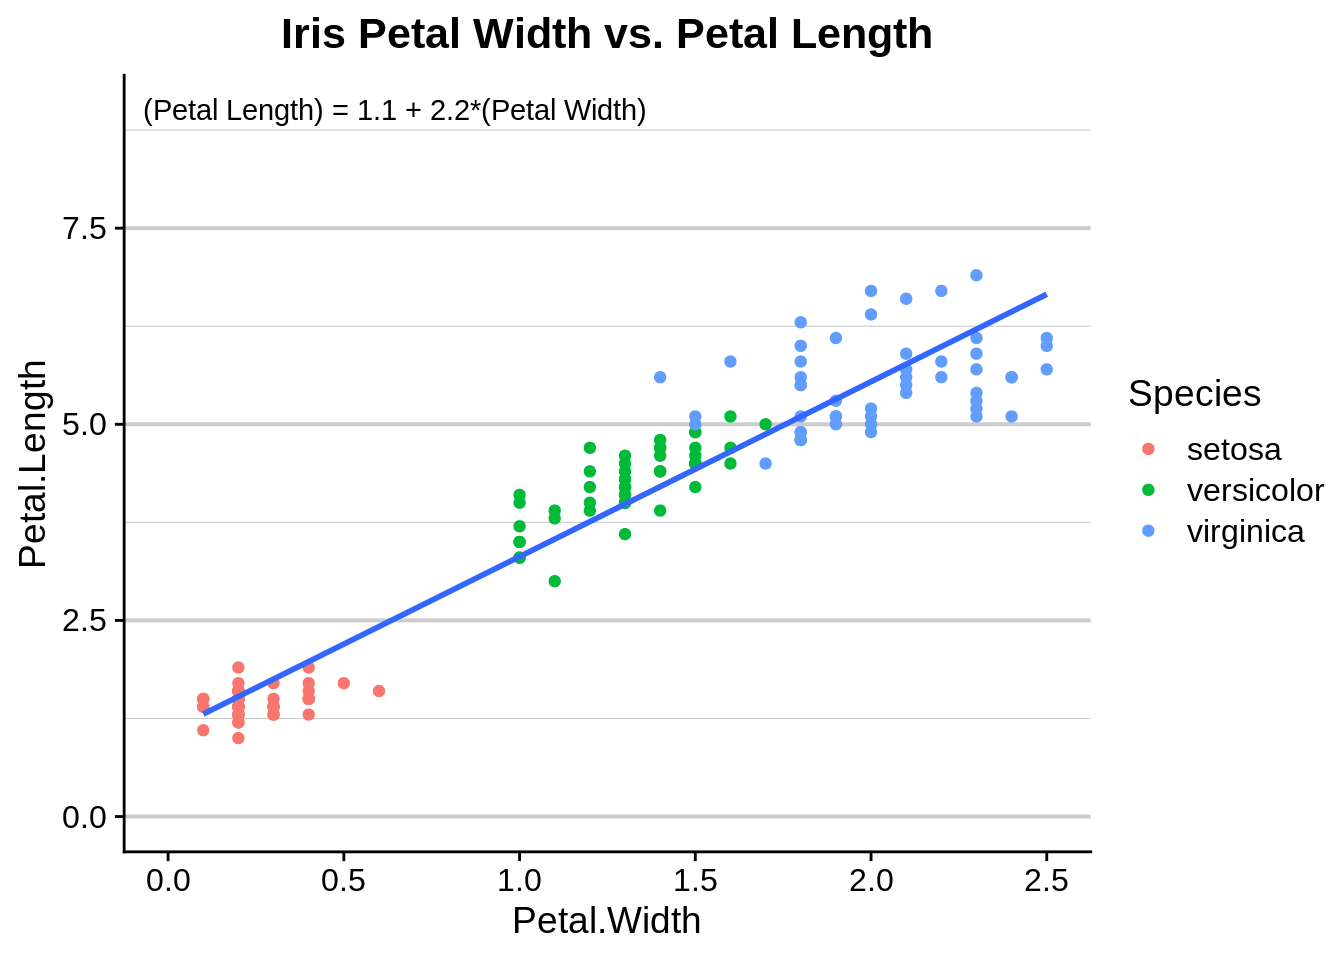
\includegraphics{Bio373L-Book_files/figure-latex/irisBad-1.pdf}
\caption{\label{fig:irisBad}Petal width (X variable) vs petal length (Y variable).
The regression is significant (\(R^2 = 0.93\); \(p<0.0001\)).}
\end{figure}

Figure \ref{fig:irisGood} contains the same data, but has been
reformatted to address these issues. Note the use of units in the axis
labels, the formatting of scientific species names, the positioning of
the legend to minimize whitespace, and the lack of a title and
gridlines. This is also an example of how to plot data with a continuous
response and a combination of continuous and categorical predictors.

\begin{figure}
\centering
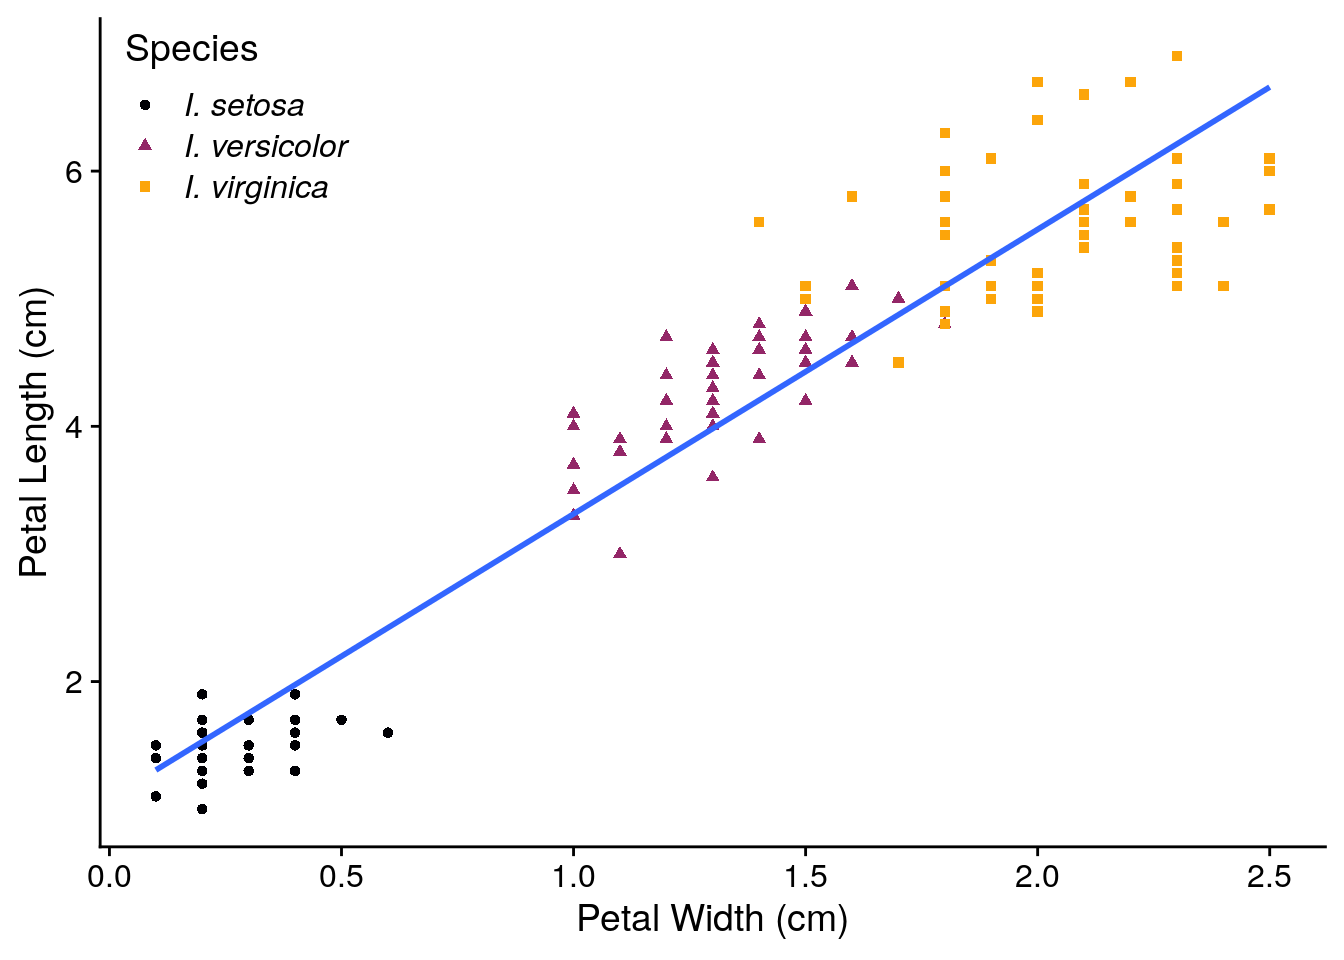
\includegraphics{Bio373L-Book_files/figure-latex/irisGood-1.pdf}
\caption{\label{fig:irisGood}Association between petal width and petal length in
three species of \emph{Iris}. Petal length increases with petal width
((Petal Length) = 1.1 + 2.2*(Petal Width); \(R^2 = 0.93\);
\(p<0.0001\)).}
\end{figure}

Figure \ref{fig:irisPanel} is an example of a multi-panel figure; in the
text, you should refer to parts of it as Figure \ref{fig:irisPanel}A,
\ref{fig:irisPanel}B, etc.






\begin{figure}
\centering
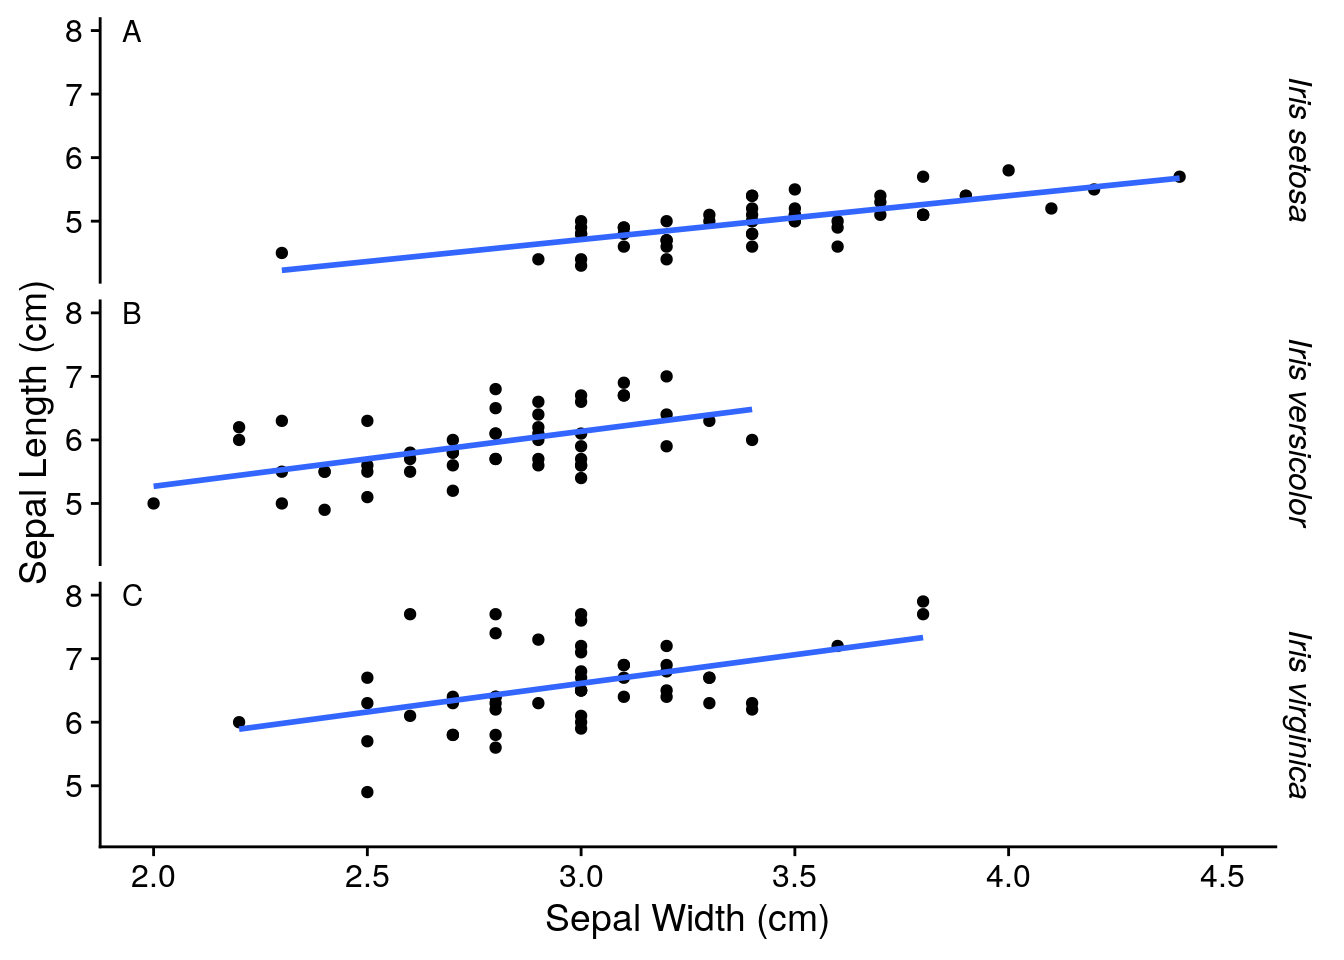
\includegraphics{Bio373L-Book_files/figure-latex/irisPanel-1.pdf}
\caption{\label{fig:irisPanel}Association between sepal width and sepal length for
A) \emph{Iris setosa}, B) \emph{I. versicolor}, and C) \emph{I.
virginica}. The association is not statistically significant ((Sepal
Length) = 6.5 + -0.2*(Sepal Width); \(R^2 = 0.01\); \(p = 0.152\)).}
\end{figure}

\subsection{Continuous response, categorical
predictors}\label{continuous-response-categorical-predictors}

There are a number of options for representing continuous data grouped
into multiple categories. You should avoid ``dynamite'' plots (Figure
\ref{fig:dynamite}), which use a bar with error lines to represent a
mean and standard error; these figures use a lot of space to provide
very little information. A better option is to use box plots (Figure
\ref{fig:boxplot}), which show the median, quartiles, range, and
outliers of each group. Equivalently, you could use a group of
histograms (Figure \ref{fig:histoplot}). A particularly effective way to
visualize this type of dataset shows the distribution of the data and
the summary statistics (Figure \ref{fig:violin}).













\begin{figure}
\centering
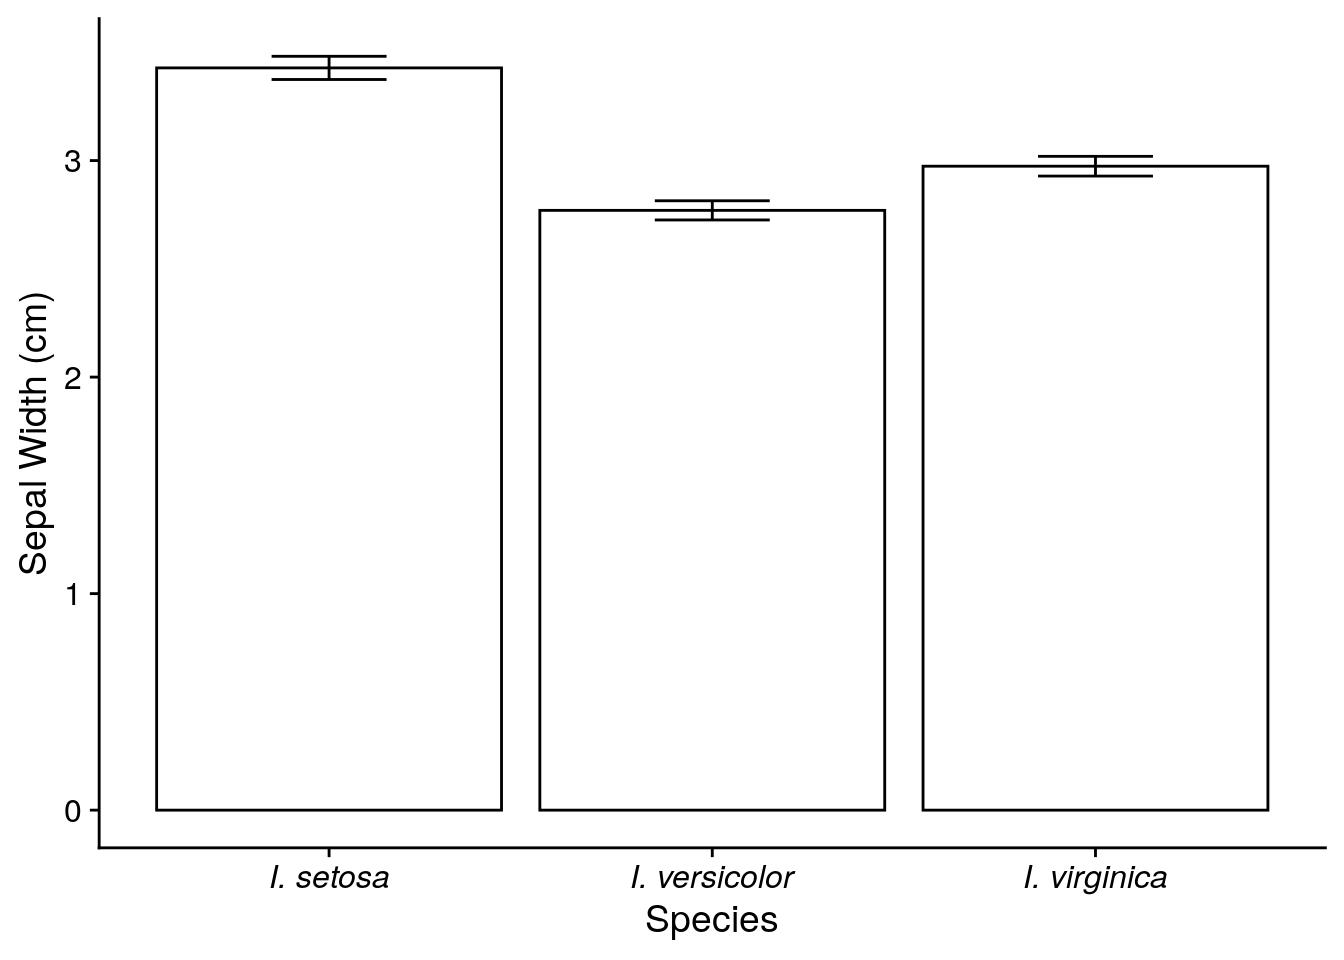
\includegraphics{Bio373L-Book_files/figure-latex/dynamite-1.pdf}
\caption{\label{fig:dynamite}Mean sepal width for three species of \emph{iris},
with standard errors. Sepal length differs significantly among species
\((p < 0.0001)\).}
\end{figure}

\begin{figure}
\centering
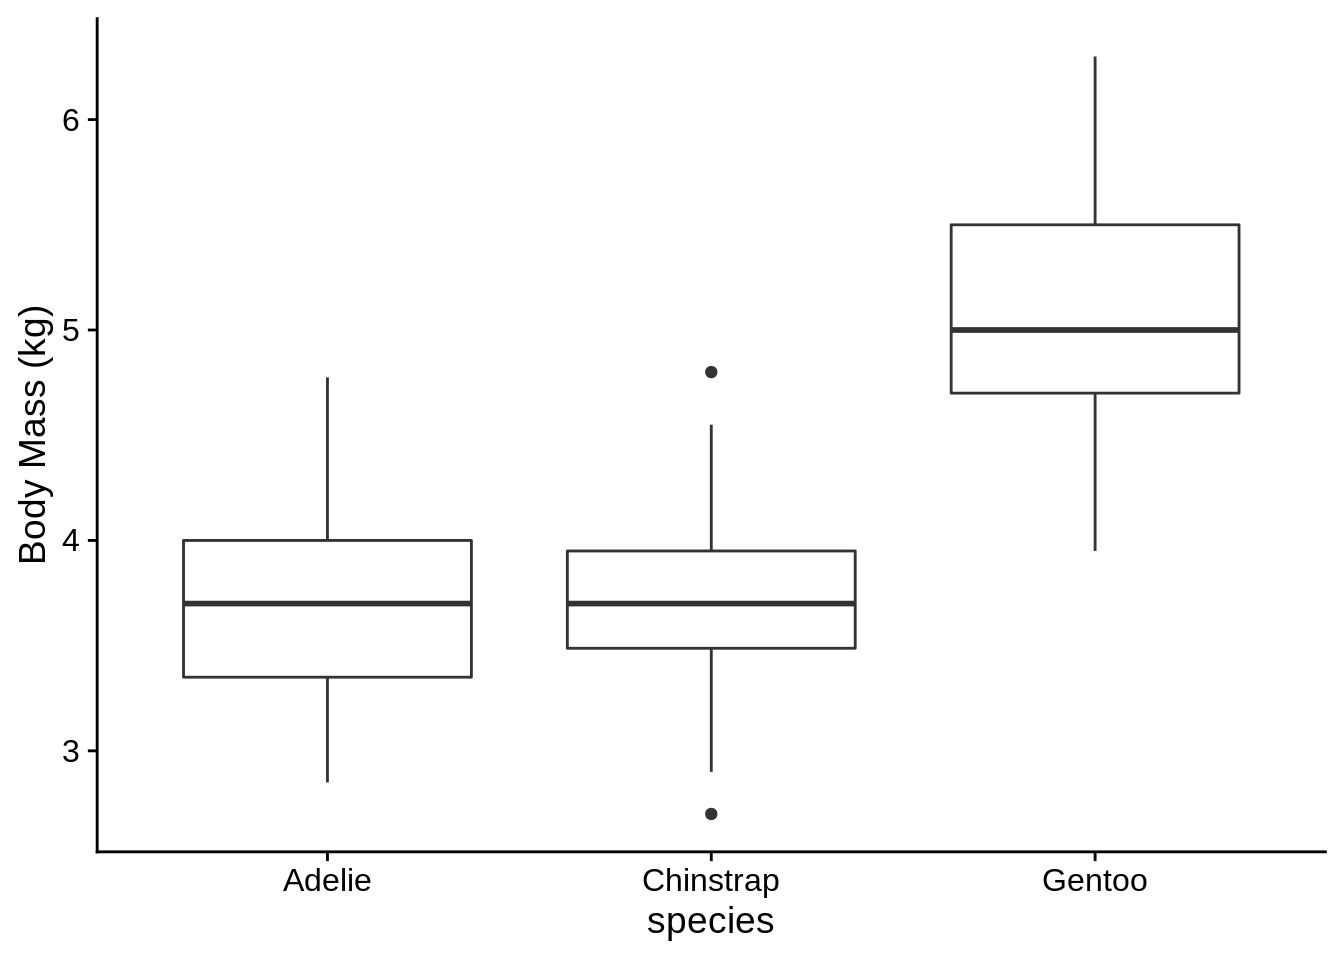
\includegraphics{Bio373L-Book_files/figure-latex/boxplot-1.pdf}
\caption{\label{fig:boxplot}Distribution of sepal width for three species of
\emph{iris}. Sepal length differs significantly among species
\((p < 0.0001)\).}
\end{figure}

\begin{figure}
\centering
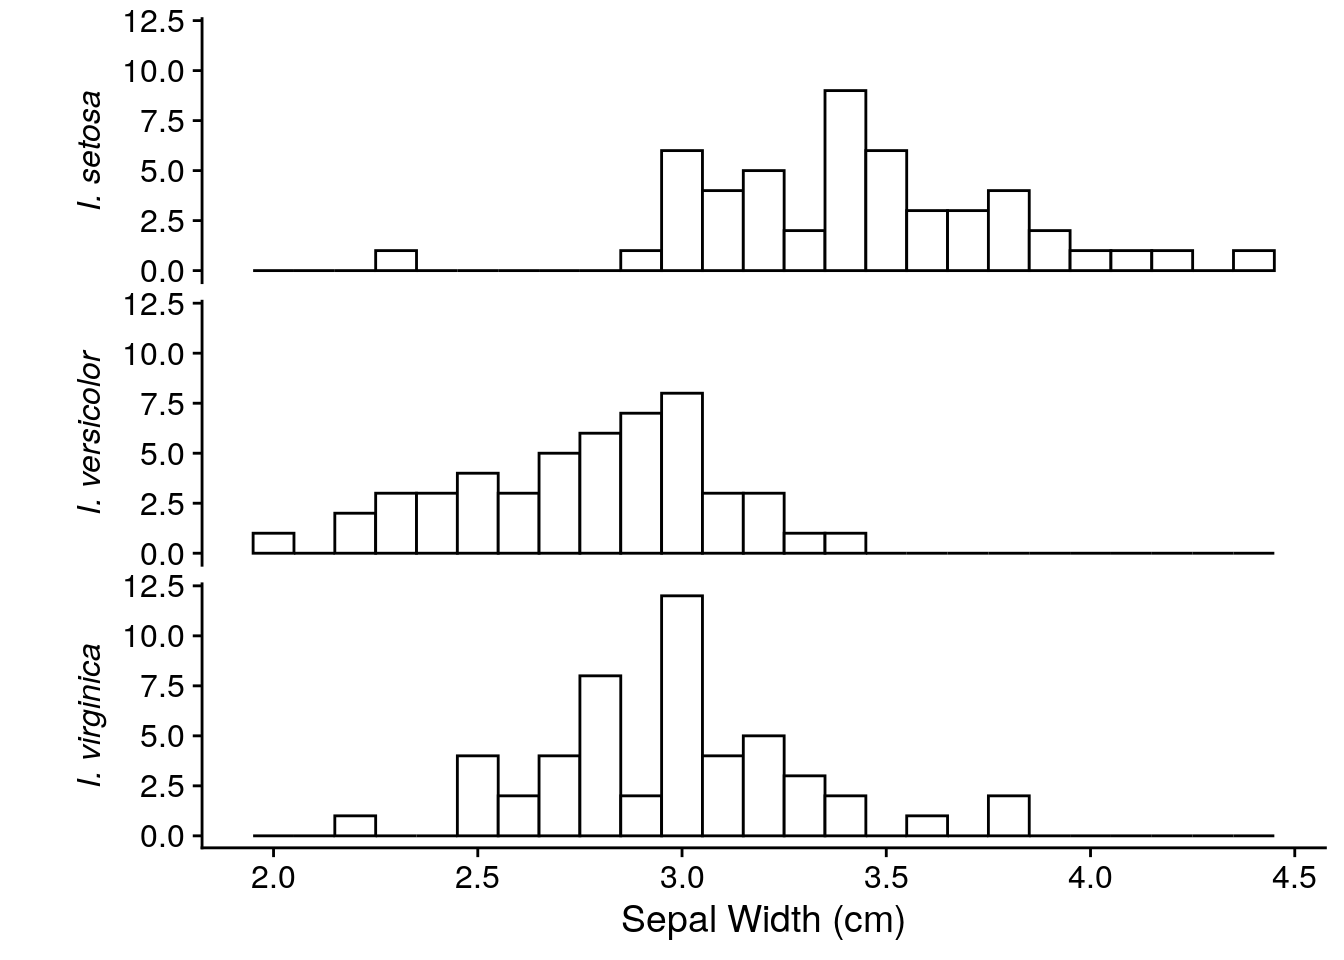
\includegraphics{Bio373L-Book_files/figure-latex/histoplot-1.pdf}
\caption{\label{fig:histoplot}Distribution of sepal width for three species of
\emph{iris}. Sepal length differs significantly among species
\((p < 0.0001)\).}
\end{figure}

\begin{figure}
\centering
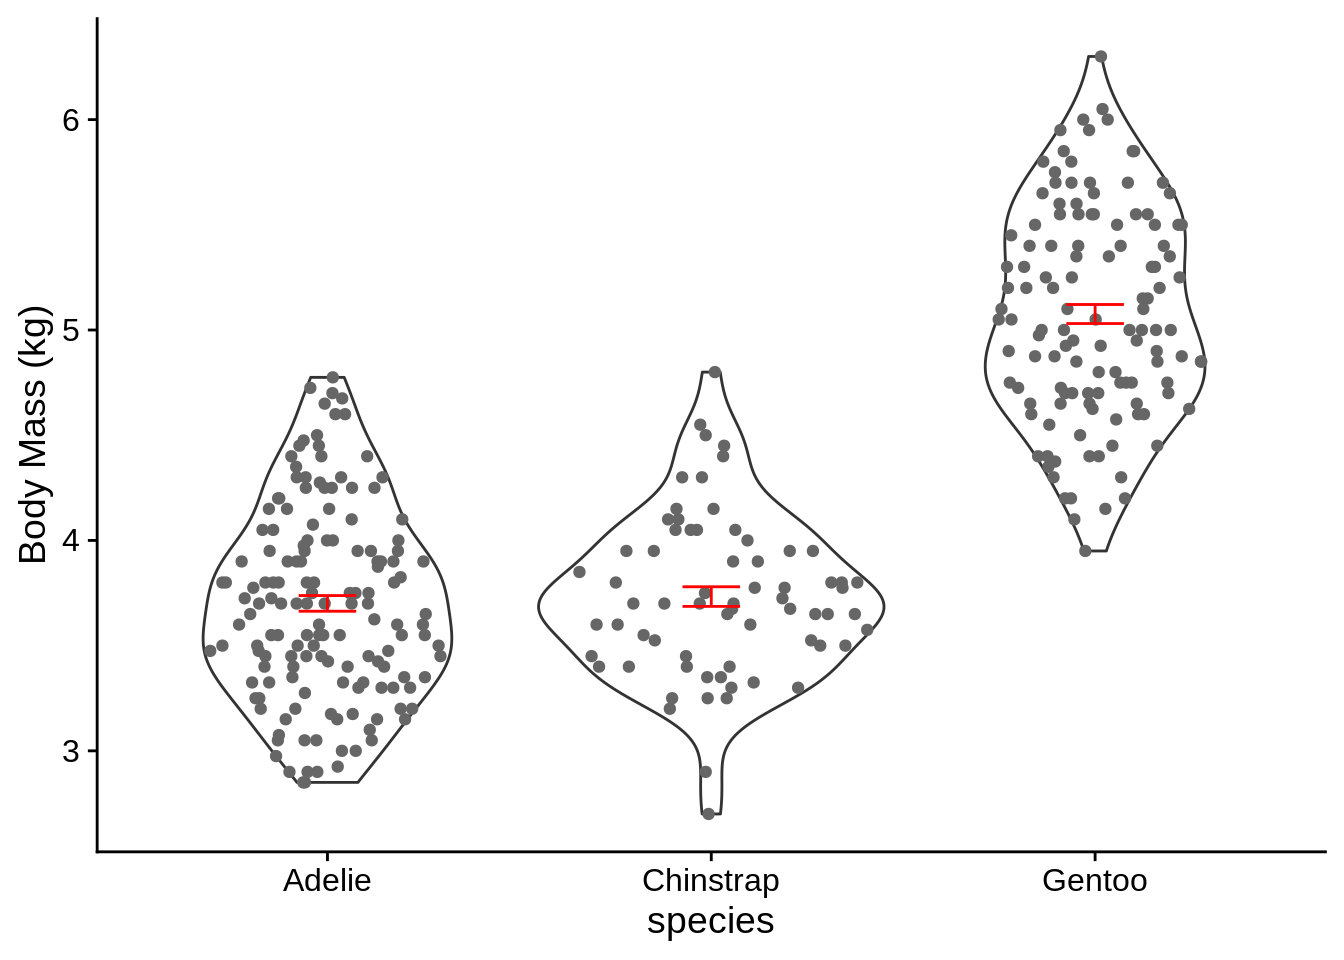
\includegraphics{Bio373L-Book_files/figure-latex/violin-1.pdf}
\caption{\label{fig:violin}Distribution of sepal width, for three species of
\emph{iris}, with mean and standard errors in red. Sepal length differs
significantly among species \((p < 0.0001)\).}
\end{figure}

\subsection{Categorical, count, or frequency
responses}\label{categorical-count-or-frequency-responses}

These sorts of data usually involve examining how counts or frequencies
differ among groups; they're often associated with \(\chi^2\) tests.
Generally, it's best to represent these sorts of data with bar graphs
(avoid pie charts). When making a bar graph, it's a good idea to arrange
your data to emphasize any trends. The species in Figure
\ref{fig:anoleBad} are organized alphabetically, which obscures any
trend. A better option is to organize by decreasing frequency of either
total counts (like in Figure \ref{fig:anoleCountStack}) or of one of the
groups (Figure \ref{fig:anoleCountDodge}). These make it easier to
detect patterns.




\begin{figure}
\centering
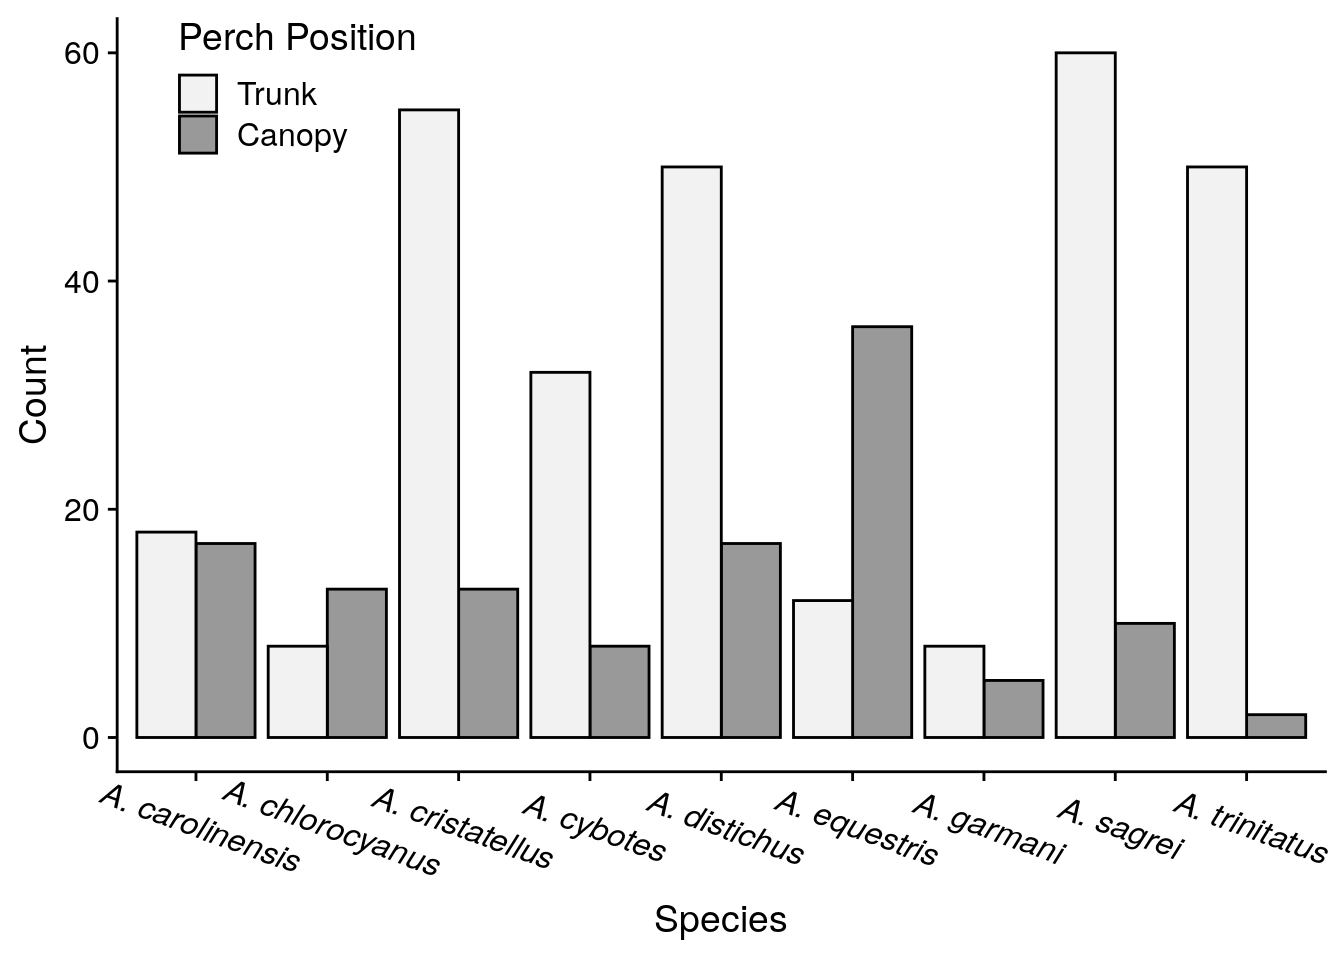
\includegraphics{Bio373L-Book_files/figure-latex/anoleBad-1.pdf}
\caption{\label{fig:anoleBad}Number of \emph{Anolis} captured from canopy and
trunk perches.}
\end{figure}

\begin{figure}
\centering
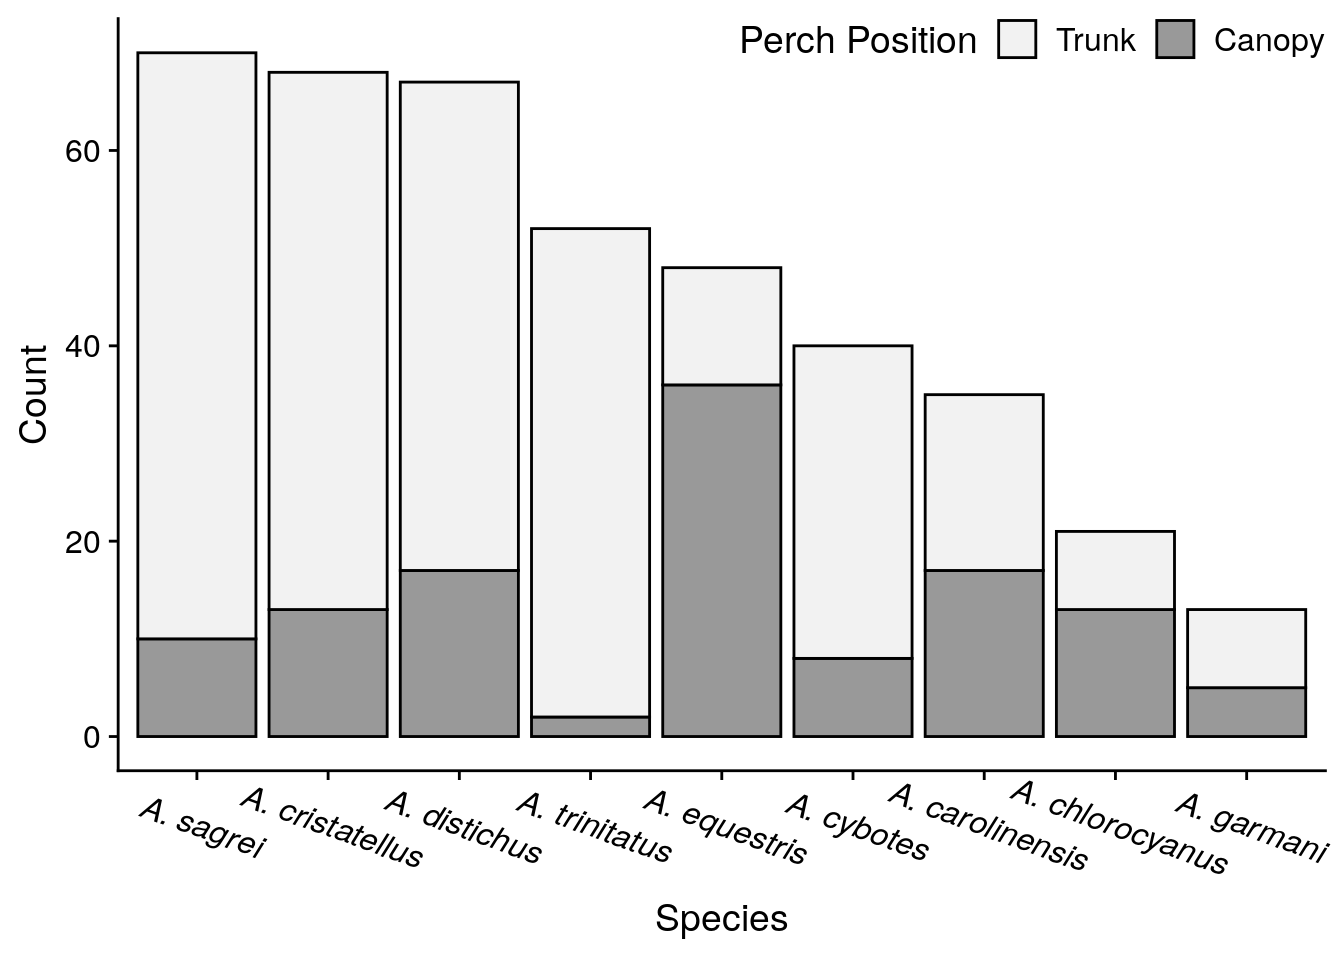
\includegraphics{Bio373L-Book_files/figure-latex/anoleCountStack-1.pdf}
\caption{\label{fig:anoleCountStack}Number of \emph{Anolis} captured from canopy and
trunk perches.}
\end{figure}

\begin{figure}
\centering
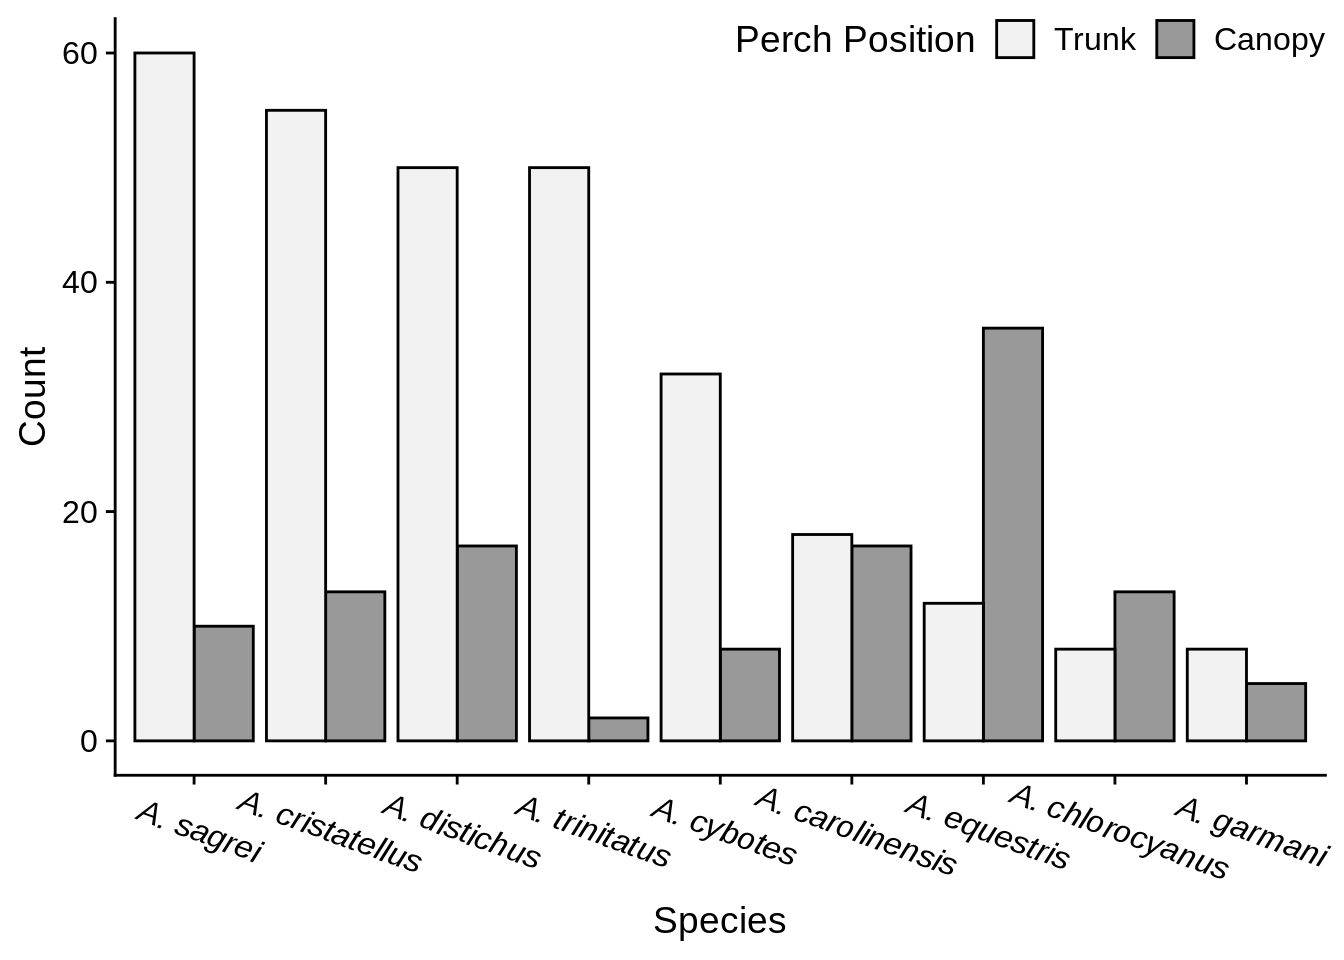
\includegraphics{Bio373L-Book_files/figure-latex/anoleCountDodge-1.pdf}
\caption{\label{fig:anoleCountDodge}Number of \emph{Anolis} captured from canopy and
trunk perches.}
\end{figure}

An important consideration is whether to represent your data with counts
or proportions (AKA frequencies -- vary from 0 to 1). There are pros and
cons to both approaches, but frequencies are usually better if the
number of observations differs among your groups (compare Figure
\ref{fig:anoleFreqByPerch} with Figure \ref{fig:anoleCountDodge}). Be
careful when calculating frequencies, because you may inadvertently end
up making a graph that isn't answering the question you're trying to
ask. For example, Figure \ref{fig:anoleFreqByPerch} shows how anole
frequencies differ between perch types, but Figure
\ref{fig:anoleFreqBySpp} shows the frequency at which each species
occupies the two perches.




\begin{figure}
\centering
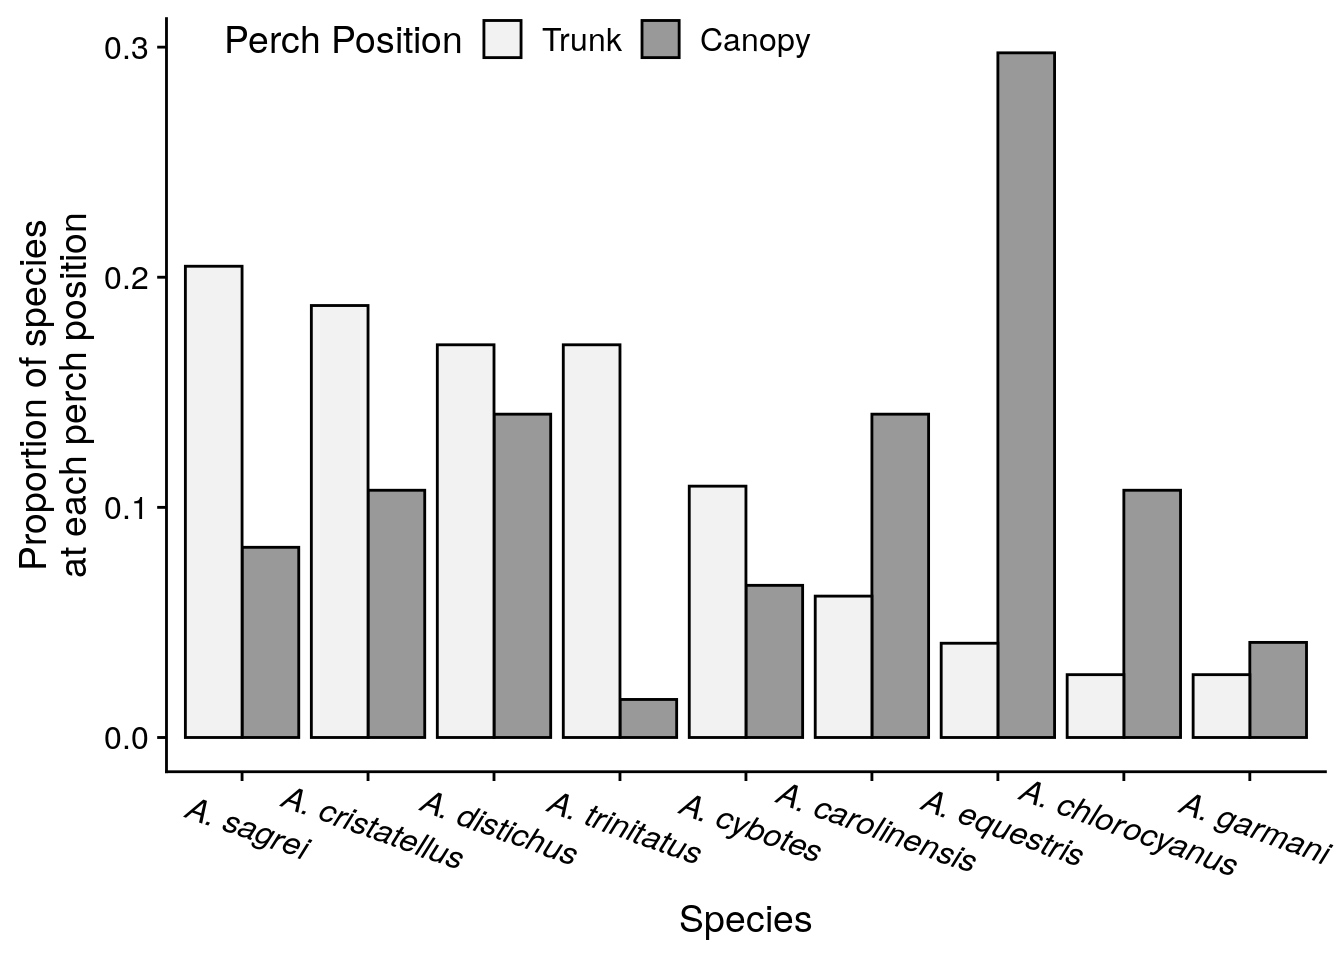
\includegraphics{Bio373L-Book_files/figure-latex/anoleFreqByPerch-1.pdf}
\caption{\label{fig:anoleFreqByPerch}Frequency of \emph{Anolis} species captured from
canopy and trunk perches.}
\end{figure}



\begin{figure}
\centering
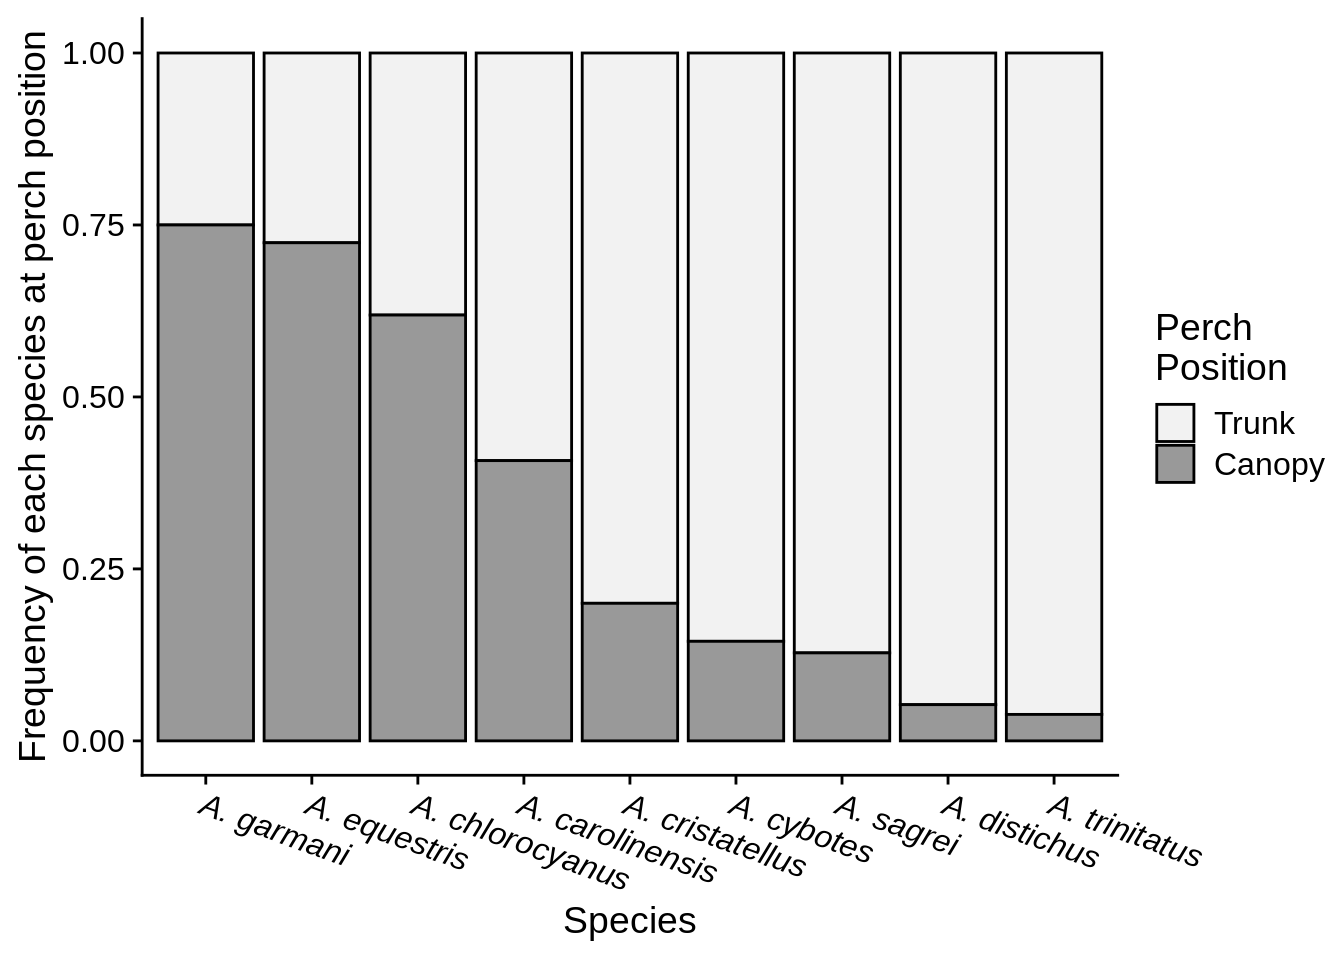
\includegraphics{Bio373L-Book_files/figure-latex/anoleFreqBySpp-1.pdf}
\caption{\label{fig:anoleFreqBySpp}Perch frequency for 9 species of \emph{Anolis}.}
\end{figure}

If there is some aspect of your data that you'd like to really
emphasize, it can help to get more creative with your figures. For
example, the most visually striking parts of Figure
\ref{fig:anoleBarFreqDiff} are the colored sections of the bars, which
correspond to the direction and magnitude of the difference between
perches for each species. Do note that making more complicated figures
may require extra explanation in the caption.







\begin{figure}
\centering
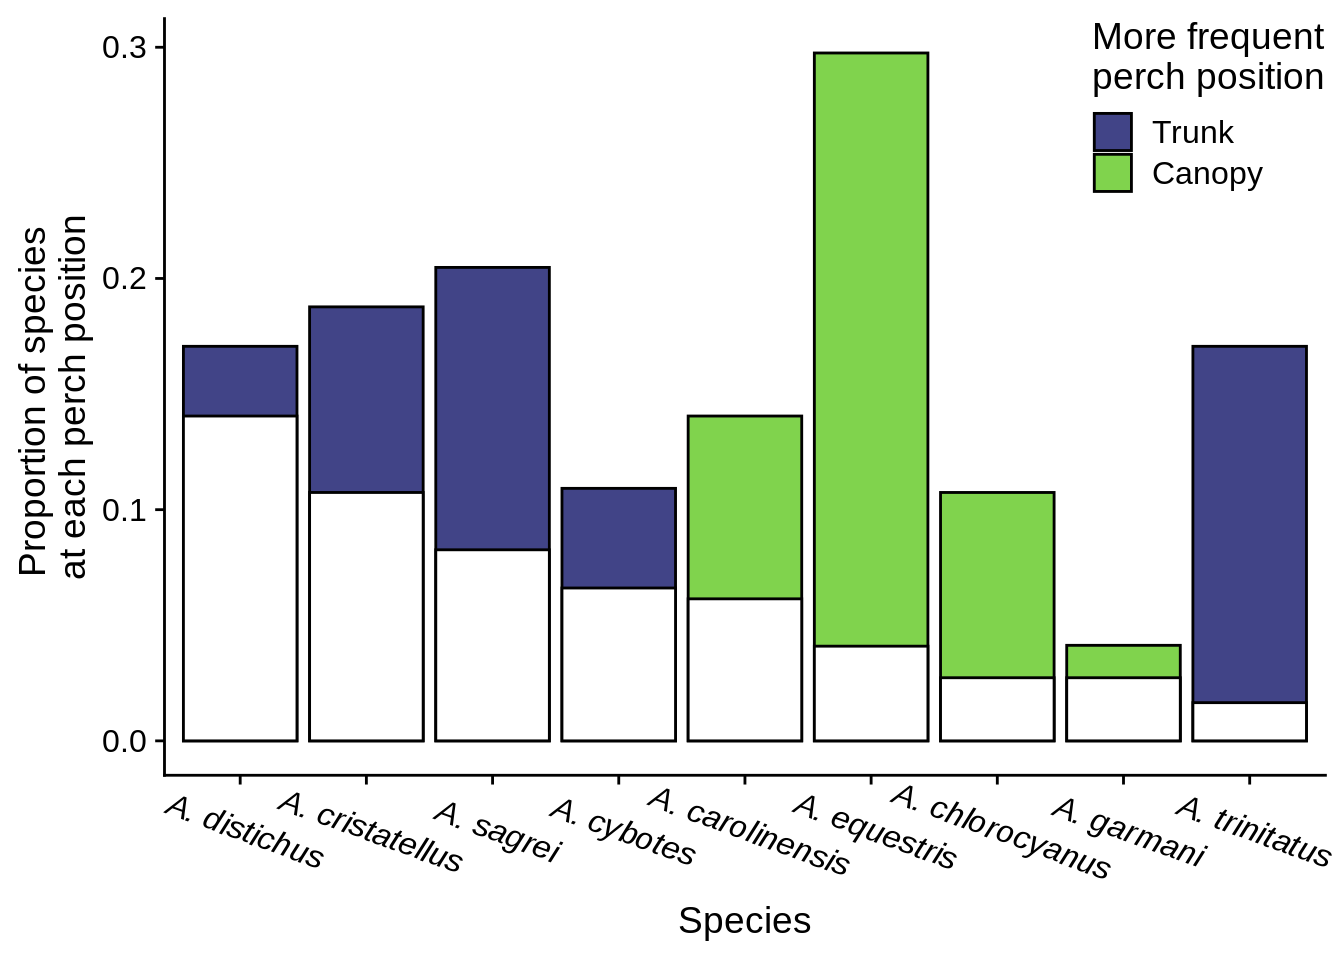
\includegraphics{Bio373L-Book_files/figure-latex/anoleBarFreqDiff-1.pdf}
\caption{\label{fig:anoleBarFreqDiff}Number of \emph{Anolis} found at each perch position.
The white bar indicates the count at the less frequent perch, the total
height is the count at the more frequent perch, color indicates which
perch the species was more common at, and the size of the colored
regions indicates the difference between perches.}
\end{figure}

\section{Tables}\label{tables}

Tables are an effective addition to a manuscript when you have a lot of
data in the text and want to present it to the reader in an organized
fashion. They are particularly helpful when you have a lot of different
kinds of data that would be hard to plot together. For example, see
Table \ref{tab:table1}.

Tables are best for highly structured data. If there isn't much data to
present, the data can usually just be presented in the text of the
results. If there's a lot of data, it is worth considering if a figure
would be better.

\begin{table}

\caption{\label{tab:table1}Standard length of three populations of rainbow trout (*Oncorhynchus mykiss*) in Southern Appalachian streams.  Group A was collected from the New River, group B from the Watauga River and group C from Winkler Creek.}
\centering
\begin{tabular}[t]{lrrrrr}
\toprule
Group & N & Mean & Std. Dev. & Min. & Max.\\
\midrule
A & 10 & 35.33 & 3.53 & 30.74 & 37.02\\
B & 15 & 42.61 & 4.62 & 36.36 & 49.17\\
C & 12 & 22.00 & 2.97 & 17.99 & 26.38\\
\bottomrule
\end{tabular}
\end{table}

\chapter{Lab 1: Succession}\label{lab1}

Some guidelines

\section{Results}\label{results-2}

You should provide data and analyses to address the following questions:

\begin{itemize}
\tightlist
\item
  What are the qualitative trends and characteristics of each habitat?
\item
  How does the total density of canopy trees differ between habitats?
\item
  Does relative abundance of each species differ between canopy and
  sapling trees? How consistent is this among habitats?
\end{itemize}

\subsection{Canopy tree density}\label{canopy-tree-density}

You can use the point-quarter method to estimate tree density at each
site with a bit of math. Let \(x_i\) be the distance from your point to
a sampled canopy tree. If you sampled 4 trees at a point, then the
density in trees per square meters would be
\(\frac{4}{x_1^2 + x_2^2 + x_3^2 + x_4^2}\). More generally, the density
is \(1 / \text{mean}(x^2)\).

Calculate density for each sample point, and convert it to hectares
(multiply by \(10,000 \text{ m}^2/\text{ha}\)). How do densities compare
between habitat types? Create a figure and compare the averages. Note
that you won't be able to claim that one group is different unless you
use statistical tests, such as a one-way ANOVA (this is optional).

\subsection{Species by habitat and life
stage}\label{species-by-habitat-and-life-stage}

For each habitat, you will want to calculate the relative abundance of
each tree species for canopy and sapling trees (i.e., number of Canopy
species \emph{x} in habitat \emph{y} divided by total number of observed
Canopy trees in \emph{y}). Visualize the result for each habitat (a
three-panel frequency plot would be the best way to go, with categories
ordered by canopy abundance).

To test if the relative proportions in canopy and saplings are
equivalent, you should construct contingency tables for each habitat
(See Table \ref{tab:contingency} for an example). Restrict each table to
the five most common species in each habitat.\\
Contingency tables can be constructed with pivot tables in Excel or the
table() function in R. Use chi-square tests to see if the proportions of
species are different between canopy and saplings for each habitat.

\begin{table}

\caption{\label{tab:contingency}Abundance of most common canopy and sapling trees in the BFL old pasture habitat, Fall 2018.}
\centering
\begin{tabular}[t]{l|r|r|r|r|r|r}
\hline
  & *Carya illinoiensis* & *Celtis spp.* & *Juniperus spp.* & *Quercus buckleyi* & *Quercus fusiformis* & *Ulmus crassifolia*\\
\hline
Canopy & 7 & 2 & 17 & 3 & 2 & 9\\
\hline
Sapling & 0 & 6 & 7 & 3 & 6 & 11\\
\hline
\end{tabular}
\end{table}

\section{Discussion}\label{discussion-1}

Some suggestions for discussion topics:

\begin{itemize}
\tightlist
\item
  How could differences in sapling/canopy relative abundances inform
  possible successional trends? Based on your results, what would you
  predict about future dominant species in the habitats?
\item
  Did you observe anything else about the ecology or natural history of
  these areas that may help account for your results (e.g., drought
  stress, dead trees, invasive species, disease, etc)?
\item
  What may be driving the differences in the habitat types? Considering
  the history of BFL may be helpful in explaining some of this.
\item
  Develop a likely scenario for the past and future decades of tree
  population dynamics in the woodlands of BFL.
\item
  How has drought and oak wilt affected the tree community at BFL? How
  might a scenario for succession based on currently healthy trees be
  changed if we include the information on stressed/dead trees?
\item
  How could this line of research be expanded upon in future work?
\end{itemize}

\section{General Comments
(Post-Review)}\label{general-comments-post-review}

\subsection{Figures}\label{figures-1}

Review the guidelines in the Figures chapter. Specifically:

\begin{itemize}
\tightlist
\item
  Don't use figure titles; anything that could go there should be in the
  caption instead.
\item
  Use colors that will work in black and white,
\item
  Number figures in the order they're cited in the main text; they
  should also be arranged in this order (e.g., figure 2 shouldn't be
  placed before figure 1).
\item
  If the figure contains new data (which all of these should), it should
  be cited in the results.
\item
  Figure numbers shouldn't have decimals in them (e.g., no Figures 1.1,
  2.3, etc). If you have a multi-panel figure, refer to specific panels
  as Figure 1a, 1b, etc.
\item
  If you have a multi-panel figure, there should be a single caption
  that explains what each of the panels are.
\item
  Don't use bar plots for group means; boxplots or violin plots are
  usually better. This is a very inefficient way to present 3 data
  points, and it provides no information about the data's variability.
  Boxplots or violin plots are better options. (Note that bar plots are
  still fine for counts or proportions).
\item
  No gridlines (see below)
\end{itemize}

To remove gridlines in excel, just click on them and delete them. Base
plots in R (with the \texttt{plot()} function) shouldn't have them by
default. To remove them with \texttt{ggplot2} figures, put this near the
top of the code:

\begin{Shaded}
\begin{Highlighting}[]
\KeywordTok{install.packages}\NormalTok{(}\StringTok{"cowplot"}\NormalTok{) }\CommentTok{# if you don't have this installed; run once}
\KeywordTok{library}\NormalTok{(cowplot)}
\KeywordTok{theme_set}\NormalTok{(}\KeywordTok{theme_cowplot}\NormalTok{()) }\CommentTok{# this makes your ggplots look nicer until you restart R}
\CommentTok{# ggplot commands here}
\end{Highlighting}
\end{Shaded}

\subsection{Write this like you're trying to publish
it}\label{write-this-like-youre-trying-to-publish-it}

You should write these reports as if you were writing a manuscript for a
journal. Pretend it's not a class paper; don't say ``For this lab, our
assignment was\ldots{}'' or ``the other students\ldots{}'' Write like
it's a research project; you came up with the hypotheses and methods and
the other students in the class are your collaborators.

When describing the data collection, you need to describe how all of
this year's data was collected, for all groups. Instead of saying ``we
sampled three points in per habitat,'' say ``five groups each sampled
three points per habitat.'' As part of this, don't talk about combining
your group's data with the rest.

Finally, you need to have a real title.

\subsection{Describe the habitats}\label{describe-the-habitats}

Since the different habitat types are an important part of this paper,
you should describe them in a reasonable amount of detail; this could go
in the intro or methods section, depending on how you wrote it.

\subsection{The Analysis}\label{the-analysis}

Formally, the chi-squared test evaluates whether the rows and columns of
a contingency table are independent of each other. In the context of
this project, that's equivalent to testing whether the Canopy:Sapling
ratio was equal for each species OR if the prevalence of each species
was the same for canopy and sapling trees.

Several people misinterpreted the analysis as examining if there were
more canopy or sapling trees. This wouldn't work, because the chi-square
test cannot tell you anything about the actual number of trees and
because the way you collected the data (a fixed number of trees per
point) was not set up to answer this question.

The Chi-square analysis was often described incorrectly in the methods;
an unfamiliar reader would not know what you were testing. When you're
describing the test, you don't necessarily need to state the
null/alternative hypotheses, but you need to make it clear what question
you're answering with it.

It's also worth remembering that the data we collect is generally not
incredibly high precision. Our measurements generally don't have the
ability to distinguish between a mean density of 437.11 and 437.14;
depending on the sample size, we may not even be able to distinguish
between 437 and 442. Being overly precise doesn't help. If your p-values
are less than 0.0001, just report ``p \textless{} 0.0001.''

\subsection{Keeping things in the right
sections}\label{keeping-things-in-the-right-sections}

Many people restated the methods used for their statistical analyses in
the results. For example:

\begin{verbatim}
"I ran chi-squared tests, and they showed significant differences in the old quarry (chi-square = ..., df = ..., p = ...), the old pasture (...) and the river terrace (...)." 
\end{verbatim}

Don't do this; instead, only provide the result. A better re-work of the
above sentence would be:

\begin{verbatim}
"Species composition was significantly different between canopy and sapling trees in the old quarry (...), the old pasture (...), and the river terrace (...)."
\end{verbatim}

Don't put anything in the intro or methods that is actually a result.
Many people listed the most common species found in each habitat in
their ``study area'' sections. Since this was a major part of this lab,
listing the dominant species should be accompanied by a citation to show
evidence that this is already known. In general, if you find yourself
saying that the most common species ``were'' something, then it sounds
like you are talking about your own observations; if you say that they
``are'' or ``have been'' something, then it sounds like you're talking
about more general patterns.

\subsection{Basic style and format
rules}\label{basic-style-and-format-rules}

\begin{itemize}
\tightlist
\item
  Don't capitalize things that don't need capitalization (e.g., the
  point-quarter technique).
\item
  Most acronyms should be defined before their first use (though there
  are a few exceptions, like ANOVA).
\item
  Don't say (p-value = x), say (p = x).
\item
  If a paper has more than two authors, cite it as ``(Smith et al.,
  2009),'' not ``(Smith, Johnson, Franks, and Brown, 2009).
\end{itemize}

\subsection{Other Comments}\label{other-comments}

\begin{itemize}
\tightlist
\item
  The ``fisher test'' is properly called Fisher's exact test (with
  ``Fisher'' capitalized).
\item
  If you used a stats program for a bunch of different things (as you
  usually do w/ R or Excel), mention it at the end of the section, not
  the beginning.
\item
  RStudio is an interface for doing analysis with R; if you used it, you
  should say you did your analysis in R.
\item
  Make sure to explain that sample points were selected differently in
  pond/old pasture than in other habitats.
\item
  In the discussion, if you are listing several possible interpretations
  of your results, it's a good idea to put the most interesting one(s)
  ahead of the ``this is all random noise'' option.
\end{itemize}

\chapter{Lab 2: Woodland Heterogeneity}\label{Lab2}

\section{Questions and Hypotheses}\label{questions-and-hypotheses}

\begin{enumerate}
\def\labelenumi{\arabic{enumi}.}
\tightlist
\item
  What are the relationships between canopy, shrub, and ground cover?
\item
  How have the relative abundance of Canopy, Shrub, and Ground cover
  categories changed over time?
\item
  {[}Add one other hypothesis that you come up with{]}
\item
  Quantify the spatial mosaic: Use a map of BFL and number/color the
  canopy level at each point. Connect adjacent areas of the same number.
  If you do this by hand, scan or photograph it and include it in the
  Canvas submission.
\end{enumerate}

Note that the ``Calibration'' step in the handout isn't included in this
section; this is still something you need to do (see below), but it's a
methods validation step, not a biological hypothesis.

\section{Analysis}\label{analysis}

\subsection{Calibrating canopy
estimates}\label{calibrating-canopy-estimates}

Since most of our analyses rely on subjective measurements, it would be
good to calibrate how well the subjective category categories predict
light measurements estimated by Gap Light Analyzer? Use linear
regression on the current datasets, with subjective score as the
predictor and percent openness as the response. Note that the structure
of the data will almost certainly violate some of the assumptions of a
linear regression test. We can still do this because this isn't a
hypothesis-driven analysis, but a prediction-driven one; provide the
\(R^2\) and fit equation, but not the p-values.

To run a regression in R, modify this code:

\begin{Shaded}
\begin{Highlighting}[]
\NormalTok{regression =}\StringTok{ }\KeywordTok{lm}\NormalTok{(y }\OperatorTok{~}\StringTok{ }\NormalTok{x, }\DataTypeTok{data =}\NormalTok{ your_data_set) }\CommentTok{# adjust this for your regression}
\NormalTok{regression }\CommentTok{# this gives you the coefficients}
\KeywordTok{summary}\NormalTok{(regression) }\CommentTok{# This includes R2 values}
\CommentTok{# Note that you should go with the "Multiple R-squared," not "Adjusted R-squared"}
\end{Highlighting}
\end{Shaded}

Create a figure for this analysis corresponding to these analyses,
including the data points and trend lines. If you're using excel, please
remember that the equation that appears after you add the trendline
shouldn't be included in the resulting graph (it belongs in the caption
and main text). If you're using \texttt{ggplot} in R, you can add a
regression line to the graph by adding the following line to your figure
code:

\begin{Shaded}
\begin{Highlighting}[]
  \KeywordTok{geom_smooth}\NormalTok{(}\DataTypeTok{method =} \StringTok{"lm"}\NormalTok{, }\DataTypeTok{se =} \OtherTok{FALSE}\NormalTok{, }\DataTypeTok{color =} \StringTok{"grey"}\NormalTok{) }
  \CommentTok{# feel free to change color}
\end{Highlighting}
\end{Shaded}

One othe thing I'd recommend is spreading out the points on your x axis
a little, since otherwise they will just be four vertical lines. In
ggplot, you can do this by replacing \texttt{geom\_point} with:

\begin{Shaded}
\begin{Highlighting}[]
  \KeywordTok{geom_jitter}\NormalTok{(}\DataTypeTok{height =} \DecValTok{0}\NormalTok{, }\DataTypeTok{width =}\NormalTok{ .}\DecValTok{25}\NormalTok{) }
  \CommentTok{# changing width will spread the dots out more; just don't change height}
\end{Highlighting}
\end{Shaded}

\subsection{Relationship between canopy and ground
cover}\label{relationship-between-canopy-and-ground-cover}

Create four contingency tables examining the ground \& shrub cover
relationship; one for each level of canopy cover. Note that the cells of
the tables should be a count (number of plots), not a relative
proportion. Run chi-squared tests on each table. This is rather similar
to what you did for the previous lab.

Re-create these tables with the relative number of plots per canopy
cover type for each ground/shrub combination. You need to visually
present this information in some way; you could try making a graph of
some sort, or you could color the cells of the table to indicate the
strength of the proportion. Note that adding color information to a
table would turn it into a figure, and it should be referred to as such.

\subsection{Historical Trends}\label{historical-trends}

How have the relative abundances of each category within the three cover
types changed over time?\\
You don't need to do an analysis for this, but create a figure. Since
this data changes over time, you should have time along the x axis of
the figure.\\
Line plots and stacked box plots are two possible options.\\
Multiple panels may be warranted.

\chapter{\texorpdfstring{Lab 4: Mark-Release-Recapture with
\emph{Heliconius}}{Lab 4: Mark-Release-Recapture with Heliconius}}\label{Lab4}

\section{Questions and hypotheses}\label{questions-and-hypotheses-1}

Primary Questions:

\begin{enumerate}
\def\labelenumi{\arabic{enumi}.}
\tightlist
\item
  How does sampling intensity improve MMR estimates?
\item
  Does separating animals by sex alter our estimate of population size?
  What's the Sex ratio?
\item
  How does the Lincoln-Pearson model compare with alternate MMR methods?
\item
  Are the \emph{Heliconius} populations in Hardy-Weinberg equilbrium for
  the Optix gene?
\end{enumerate}

\subsection{Wing Pattern and the Optix transcription
factor}\label{wing-pattern-and-the-optix-transcription-factor}

In the lab, we scored the orange/red/brown wing patterns. The mimetic
phenotypes generated are key to the diversification of the genus, to
predator protection niches, and to mutualism between sympatric species
(Mullerian mimicry). The the Optix supergene locus controls expression
of a transcription factor that affects coloration in wing patterns. A
supergene locus controls expression of a transcription factor called
Optix. One allele (\(F\)) accounts for the red, orange, red or brown
scales in the distal forewing band (beyond the large wing cell). Another
allele (\(H\)) controls the presence of such scales on the hind wing
and/or on the proximal forewing in the cell region. Since the link
between phenotype and genotype is known, we can use observational data
to infer whether the population is in Hardy-Weinberg equilibrium (HWE)
for this trait.

Hardy\_Weinberg assumptions:

\begin{itemize}
\tightlist
\item
  Mating is random
\item
  No migration
\item
  No natural selection
\item
  No genetic drift (a.k.a., large populations)
\item
  No mutation
\end{itemize}

Note that while several of the above assumptions are essentially
impossible, in practice you can achieve near-HWE if migration,
selection, drift, and mutation are small/weak enough to be ignored.

\section{Analysis}\label{analysis-1}

The Lincoln-Pearson model:

If \(S_2\) is the number of individuals collected in a sample period,
\(M_1\) is total number of previously marked individuals, and \(R_2\) is
the number of marked individuals who were recaptured, then you can
estimate population size:

\[\hat{N} = \frac{S_2 M_1}{R_2}\]

\subsection{\texorpdfstring{Effect of sampling intensity on
Lincoln-Pearson \(\hat{N}\)
estimates}{Effect of sampling intensity on Lincoln-Pearson \textbackslash{}hat\{N\} estimates}}\label{effect-of-sampling-intensity-on-lincoln-pearson-hatn-estimates}

We're going to simulate increased sampling estimates by pooling together
estimates from each team. I'll be combining the the data from each group
in all possible team combinations (e.g., one team: A, B, C, \ldots{};
two teams: AB, AC, AD, \ldots{}; three teams: ABC, ABD, BCD, \ldots{}).
For each combination, you'll need to calculate the Lincoln-Pearson
population size estimate \((\hat{N})\). Create a figure showing the
effect of sample size on \(\hat{N}\).

\subsection{Sex ratios}\label{sex-ratios}

Estimate \(\hat{N}\) separately for male and female butterflies; how
does this sum compare with the estimate for all teams combined?

What is the sex ratio of the population? Does it differ from 50:50? Use
a chi-square test to test this.

\subsection{Comparison of Lincoln-Pearson with alternative
method}\label{comparison-of-lincoln-pearson-with-alternative-method}

In 1970-71, Larry Gilbert collected data on a natural population of
Heliconius in Trinidad. We will use this method to estimate population
sizes.

For each of the three sample periods, use a regression to model the
relationship between the daily recapture proportion \((x)\) and the
cumulative number of individuals marked \((y)\). Intuitively, a
recapture rate of 1.0 would suggest that you've sampled pretty much the
entire population; you could thus use this regression equation to
estimate \((\hat{N})\) by evaluating it when \(x=1\). Create a
multi-panel regression plot to go along with these methods.

Compare these estimates with the Lincoln-Pearson estimate from the day
with the highest proportion of recaptures in the sampling period. Note
that for each row of the Trinidad data, \(S_2\) =
\texttt{total\_captured}, \(R_2\) = \texttt{recaptures}, and \(M_1\) =
\texttt{(cumulative\_m\ -\ new\_captures)}.

\subsection{Hardy-Weinberg}\label{hardy-weinberg}

First, you'll want to get the observed numbers for each genotype; we'll
call these \(N_{FF}\), \(N_{FH}\), and \(N_{HH}\); the total sample size
\(N\) is the sum of these. You can use the \texttt{table} command in R
to calculate this.

From these observed genotypes, you can calculate the genotype frequency
of F, which is just \(\frac{N_{FF} + 0.5 N_{FH} }{N}\) let's call this
\(p\).

You can get your HWE expected genotypes by using \(p\) and \(q=1-p\) to
get your expected genotype frequencies, then multiplying them by \(N\)
to get your expected counts.

From here, you have observed and expected counts and can run an
chi-square test.

\section{Discussion}\label{discussion-2}

You should address the following in your discussion:

\begin{itemize}
\tightlist
\item
  Our MMR data came from a closed population; briefly speculate about
  some of the potential problems with these estimates in an open,
  natural population (how would emigration/immigration or birth/death
  affect the estimates)? How might our study compare with data from a
  natural population?
\item
  How well does the Lincoln-Pearson model compare with fractional
  reacpture estimation in a naural population? How different were your
  population estimates? What factors could help explain them?
\item
  Think of some creative ways you could improve sampling in an MMR
  project? (Beyond just increasing the sample size).\\
\item
  Don't forget to discuss your results from the sex ratio and genotype
  analyses.
\end{itemize}

\chapter{Lab 5: Ant Community Ecology}\label{Lab5}

\section{Questions and hypotheses}\label{questions-and-hypotheses-2}

There are two primary topics we'll be investigating in this lab:

\begin{itemize}
\tightlist
\item
  What are the habitat preferences of imported fire ants
  (\emph{Solenposis invicta})?
\item
  How do ant communities differ across habitats?
\end{itemize}

\section{Analysis}\label{analysis-2}

We'll be doing examining habitat differences with a couple of contrasts
with our various methods:

\begin{itemize}
\tightlist
\item
  Open (canopy cover 0 or 1) vs.~Closed (canopy cover 2 or 3) canopies.
\item
  Sparse (0/1) vs.~dense (2/3) ground cover.
\item
  Low vs.~high disturbance
\item
  Habitat types (Q/R/P)
\end{itemize}

\subsection{\texorpdfstring{\emph{S. invicta} habitat
preference}{S. invicta habitat preference}}\label{s.-invicta-habitat-preference}

Compare the presence/absense of \emph{S. invicta} for each contrast. For
each, create a contingency table and run a chi-squared test. The columns
should be the different habitat conditions; the table should have two
rows (fire ants present, fire ants absent), and the cell contents should
be the number of baits that meet those conditions.

You should also test if there's an interaction between canopy openness
and disturbance (re: fire ant presence). This should also be tested with
a chi-square test, with the contingency table's columns being the four
combinations of openness and disturbance.

\subsection{Ant community differences}\label{ant-community-differences}

We'll be using four methods to estimate and compare diversity of ants in
different habitats at BFL: Jaccard's index of similarity, Cumulative
curves of species, Rank abundance curves and Shannon's index of
diversity. You can read about these methods in the Ecology Laboratory
Manual by G.W. Cox or any other ecology book.

In general, you should use these methods to compare the above habitat
characteristics. You don't have to do all of them for each method (that
would be excessive), but I'd recommend using them to explore the data
and report on some contrasts that you find interesting. For everything
but the Jaccard, you should also look at the entire dataset as a whole.~

\subsubsection{Jaccard's index of
similarity}\label{jaccards-index-of-similarity}

This index provides an estimation of how similar species composition is
between two communities (e.g., two places or times).

\[J = \frac{W}{A + B - W}\] \(A\) and \(B\) are the richness (number of
species present) of the two communities in question, and \(W\) is the
number of species in common in both communities. \(J\) varies from 0
(nothing in common) to 1 (identical communities). You can also interpret
\(J\) as the proportion of total species that are shared.

For these analyses, you should treat the community as the

\subsubsection{Species Accumulation
Curve}\label{species-accumulation-curve}

These curves show the amount of time/effort spent sampling for species
against the total number of species observed. They provide information
about the actual and potential species richness of a community, as well
as a sense of how well a place has been sampled. The details of how to
calculate this are a bit complicated, and are explained in the attached
R script.

Plot each curve (for related curves, you should include them in the same
figure). Does it appear that the habitat was fully sampled? Estimate the
likely number of species in the habitat by extrapolating the curve.

\subsubsection{Rank Abundance Curve}\label{rank-abundance-curve}

Rank abundance curves compare the abundance of each species to the
rank-order of that abundance. These give you a visual representation of
species richness and species evenness (measure of comparative relative
abundance of species). Species evenness is derived from the slope of the
line that fits the graph. A steep drop-off indicates low evenness as the
high ranking species have much higher abundances than the low ranking
species. A more gradual slope indicates high evenness as the abundances
of different species are similar.

To create these, plot the~number of ants found in each species with
log10 scale on Y-axis. Organize the species along the x-axis from most
to least abundant (See more in Cox pg 197).

\subsubsection{Shannon Index}\label{shannon-index}

This index estimates the diversity of a species in a single place,
combining information about the richness and relative abundance. The
Shannon index \((H^\prime)\) is calculated as:

\[H^{\prime} = -\sum_{i=1}^n p_i \ln(p_i)\] where \(p_i\) is the
relative abundance of species \(i\). The larger \(H^{\prime}\), the
higher the diversity. The exponential of the Shannon index is called the
true Shannon diversity \((D_H = \exp(H^\prime))\); it can be interpreted
as the number of species you'd expect in an equally diverse community
that was perfectly even.

\section{Discussion}\label{discussion-3}

In progress. This is a test.

\bibliography{book.bib,packages.bib}

\end{document}
